\chapter{Aplicación: Canal de vacío rodeado por Agua}

En este capítulo se presenta una aplicación del método desarrollado para la generación de fuentes Monte Carlo mediante histogramas multidimensionales. El caso de estudio seleccionado consiste en un canal de vacío rodeado lateralmente por un bloque de agua liviana, simulando de forma aproximada una guía de neutrones. El objetivo del análisis es evaluar el desempeño del método propuesto en la generación de fuentes intermedias, con el fin de mejorar la estadística del flujo escalar en regiones específicas del modelo. (y conservar la corriente.)

Para ello, se realizaron varias etapas de simulación. Inicialmente, se efectuó una simulación para registrar un archivo de partículas (trackfile) en una superficie intermedia. Posteriormente, se llevó a cabo una simulación más extensa desde la entrada del sistema hasta otra superficie más alejada, con el propósito de obtener con precisión la distribución del flujo escalar a lo largo del canal, así como la corriente y el espectro neutrónico incidente sobre esta superficie final.

Finalmente, se procesó el trackfile grabado en la superficie intermedia para construir una fuente basada en histogramas multidimensionales. Esta fuente se utilizó en una tercera simulación iniciada directamente desde la posición intermedia, obteniendo así una estadística suficientemente convergida hasta la superficie más alejada. Esta última simulación permitió realizar una comparación directa con los resultados obtenidos en la simulación extensa desde la entrada, evaluando así la eficacia y precisión del método de generación de fuentes implementado.

\section{Descripción del modelo simulado en OpenMC}

El modelo utilizado en las simulaciones consiste en un canal interno de vacío rodeado lateralmente por un bloque de agua liviana. El sistema se diseñó como un paralelepípedo de agua con dimensiones $15\,\text{cm} \times 15\,\text{cm} \times 100\,\text{cm}$, que alberga en su interior un canal de vacío con sección transversal cuadrada de $3\,\text{cm} \times 3\,\text{cm}$, orientado en dirección del eje $z$.

La fuente de neutrones utilizada se definió sobre la cara de entrada del sistema (ubicada en $z = 0,\text{cm}$) y consistió en neutrones monoenergéticos con energía de $E = 1\,\text{MeV}$ y colimados en dirección del eje $z$ (con coseno direccional $\mu = \cos(\theta) = 1$). Esta configuración genera dos poblaciones de neutrones claramente diferenciadas: la primera, formada por neutrones que atraviesan el canal de vacío sin colisiones y mantienen tanto su energía inicial como su dirección; y la segunda, constituida por neutrones que interactúan con el moderador de agua, sufriendo dispersión angular y pérdida energética.

Para el análisis y posterior generación de la fuente, se registró un trackfile sobre una superficie intermedia situada en $z = 15\,\text{cm}$. Este archivo contiene información sobre ambas poblaciones mencionadas, es decir, neutrones no colisionados y neutrones dispersados.

Durante las simulaciones se emplearon tallies para determinar el flujo escalar neutrónico a lo largo del canal, tanto dentro del canal de vacío como en el moderador circundante.

Para optimizar la estadística en regiones con baja presencia de partículas, particularmente en el agua, se implementó la técnica de ventanas de peso adaptativo disponible en OpenMC. Este método actualiza dinámicamente los pesos de las partículas durante la simulación, permitiendo obtener mejores estadísticas con partículas de peso estadístico reducido.


\section{Procesamiento del trackfile}
\subsection{Metodología del análisis}
\label{sec:metodologia-analisis}

% Para validar el método propuesto, se remuestrearon \emph{trackfiles} generados en simulaciones Monte Carlo previas y se compararon los \emph{trackfiles} obtenidos contra los originales. Estos archivos constituyen conjuntos de datos representativos que permiten verificar si la metodología implementada es capaz de aproximar adecuadamente las distribuciones y correlaciones originales del espacio de fases ($\mathbf{E}$–$\mathbf{r}$–$\boldsymbol{\Omega}$).

La estrategia general consiste en aplicar el método al \emph{trackfile} registrado, utilizando distintos esquemas de configuración. En cada configuración se varían los parámetros: el tipo de bineado, el número de macrogrupos y microgrupos, y la posibilidad de indicar bordes de macrogrupo manualmente, y se analiza su impacto en la calidad de la reconstrucción. Para definir manualmente los bordes de los macrogrupos es necesario obtener información previa sobre la geometría o el comportamiento de las partículas que permita mejorar la separación de poblaciones con características distintas.

Los principales aspectos del análisis son:

\begin{itemize}
    % \item \textbf{Orden de variables:} se considera cómo el orden en que se procesan las variables afecta a la fragmentación del \emph{trackfile} original en subconjuntos y, por ende, a la estadística de cada variable de procesamiento, que disminuye a medida que aumentan los macrogrupos. En general, la primera variable se beneficia de la estadística total, debido a que todavía no se ha subdividido en sucesivos subconjuntos, mientras que las siguientes reciben subconjuntos progresivamente más pequeños. Dado que la variable $\phi$ suele presentar una distribución cercana a uniforme en sistemas con simetría, se ha elegido colocarla en la última posición.
    
    \item \textbf{Bineado uniforme vs. adaptativo:} se comparan histogramas de igual ancho y adaptativos. A su vez, para mejorar la representación del espacio de fase $\textbf{E}$–$\textbf{r}$–$\boldsymbol{\Omega}$, se analiza el efecto de incorporar bordes de macrogrupos definidos manualmente al caso de bineado uniforme. Esto permite ajustar la segmentación de los macrogrupos a la geometría del sistema o al comportamiento esperado de las partículas, mejorando la separación entre poblaciones y, por ende, la calidad del remuestreo.

    \item \textbf{Cantidad de macrogrupos:} se comparan esquemas uniformes (por ejemplo, $[8,8,8,8]$, $[6,6,6,6]$) y esquemas crecientes o decrecientes (como $[9,8,7,6]$, $[6,7,8,9]$). Esta elección impacta en la capacidad de representar correlaciones sin introducir exceso de ruido estadístico.
    
    \item \textbf{Cantidad de microgrupos:} se estudia el efecto de aumentar o disminuir la resolución dentro de cada macrogrupo.
    
\end{itemize}

Para cada configuración de entrada se comparan visualmente las distribuciones 1D y 2D obtenidas, analizando las distribuciones y sus errores relativos, como así también se analiza la divergencia KL obtenida para los casos 1D y 2D.

\begin{itemize}
    \item \textbf{Distribuciones 1D}: se comparan las distribuciones de cada variable remuestreadas utilizando el método implementado contra las originales del \emph{trackfile}. 
    \item \textbf{Correlaciones 2D}: se representan visualmente mediante mapas de error relativo entre las matrices de correlación originales y las reconstruidas a través del remuestreo.
    \item \textbf{Métrica cuantitativa}: se utiliza la divergencia de Kullback-Leibler (KL) como estimador numérico de la diferencia entre las distribuciones, permitiendo comparar configuraciones de forma objetiva.
\end{itemize}

% En algun momento hay que explicar que el KL requiere que no haya valores 0 y requiere discretizar la muestra. Lo que se hizo fue sumarle 1e-9 a todos los bines antes de normalizar. Es tecnica de pseudoconteo. Además se han tomado 1000 bines para los casos 1D y 1000x1000 bines para los casos 2D. esto se ha dejado fijo porque al variar estos parametros valia la salida del KL. Por lo tanto para poder comparar entre distintos casos se ha dejado fijo.

\subsection{Descripción del trackfile}

El \emph{trackfile} analizado fue registrado en una primera simulación del tubo de vacío desde el comienzo de la geometría. Corresponde a partículas registradas en una superficie ubicada a 15cm del inicio de la geometría. La lista contiene tanto neutrones que atraviesan la sección del canal, como neutrones que viajan por el agua. Sin embargo, la mayor proporción de peso estadístico se encuentra dentro del tubo de vacío, lo cual se corrobora en la proyección $x$-$y$, donde se observa una distribución más intensa contenida en un cuadrado correspondiente a la sección del tubo. La figura \ref{fig:trackfile1_x_y} muestra la proyección de los neutrones en el plano $x$-$y$.

\begin{figure}[H]
    \centering
    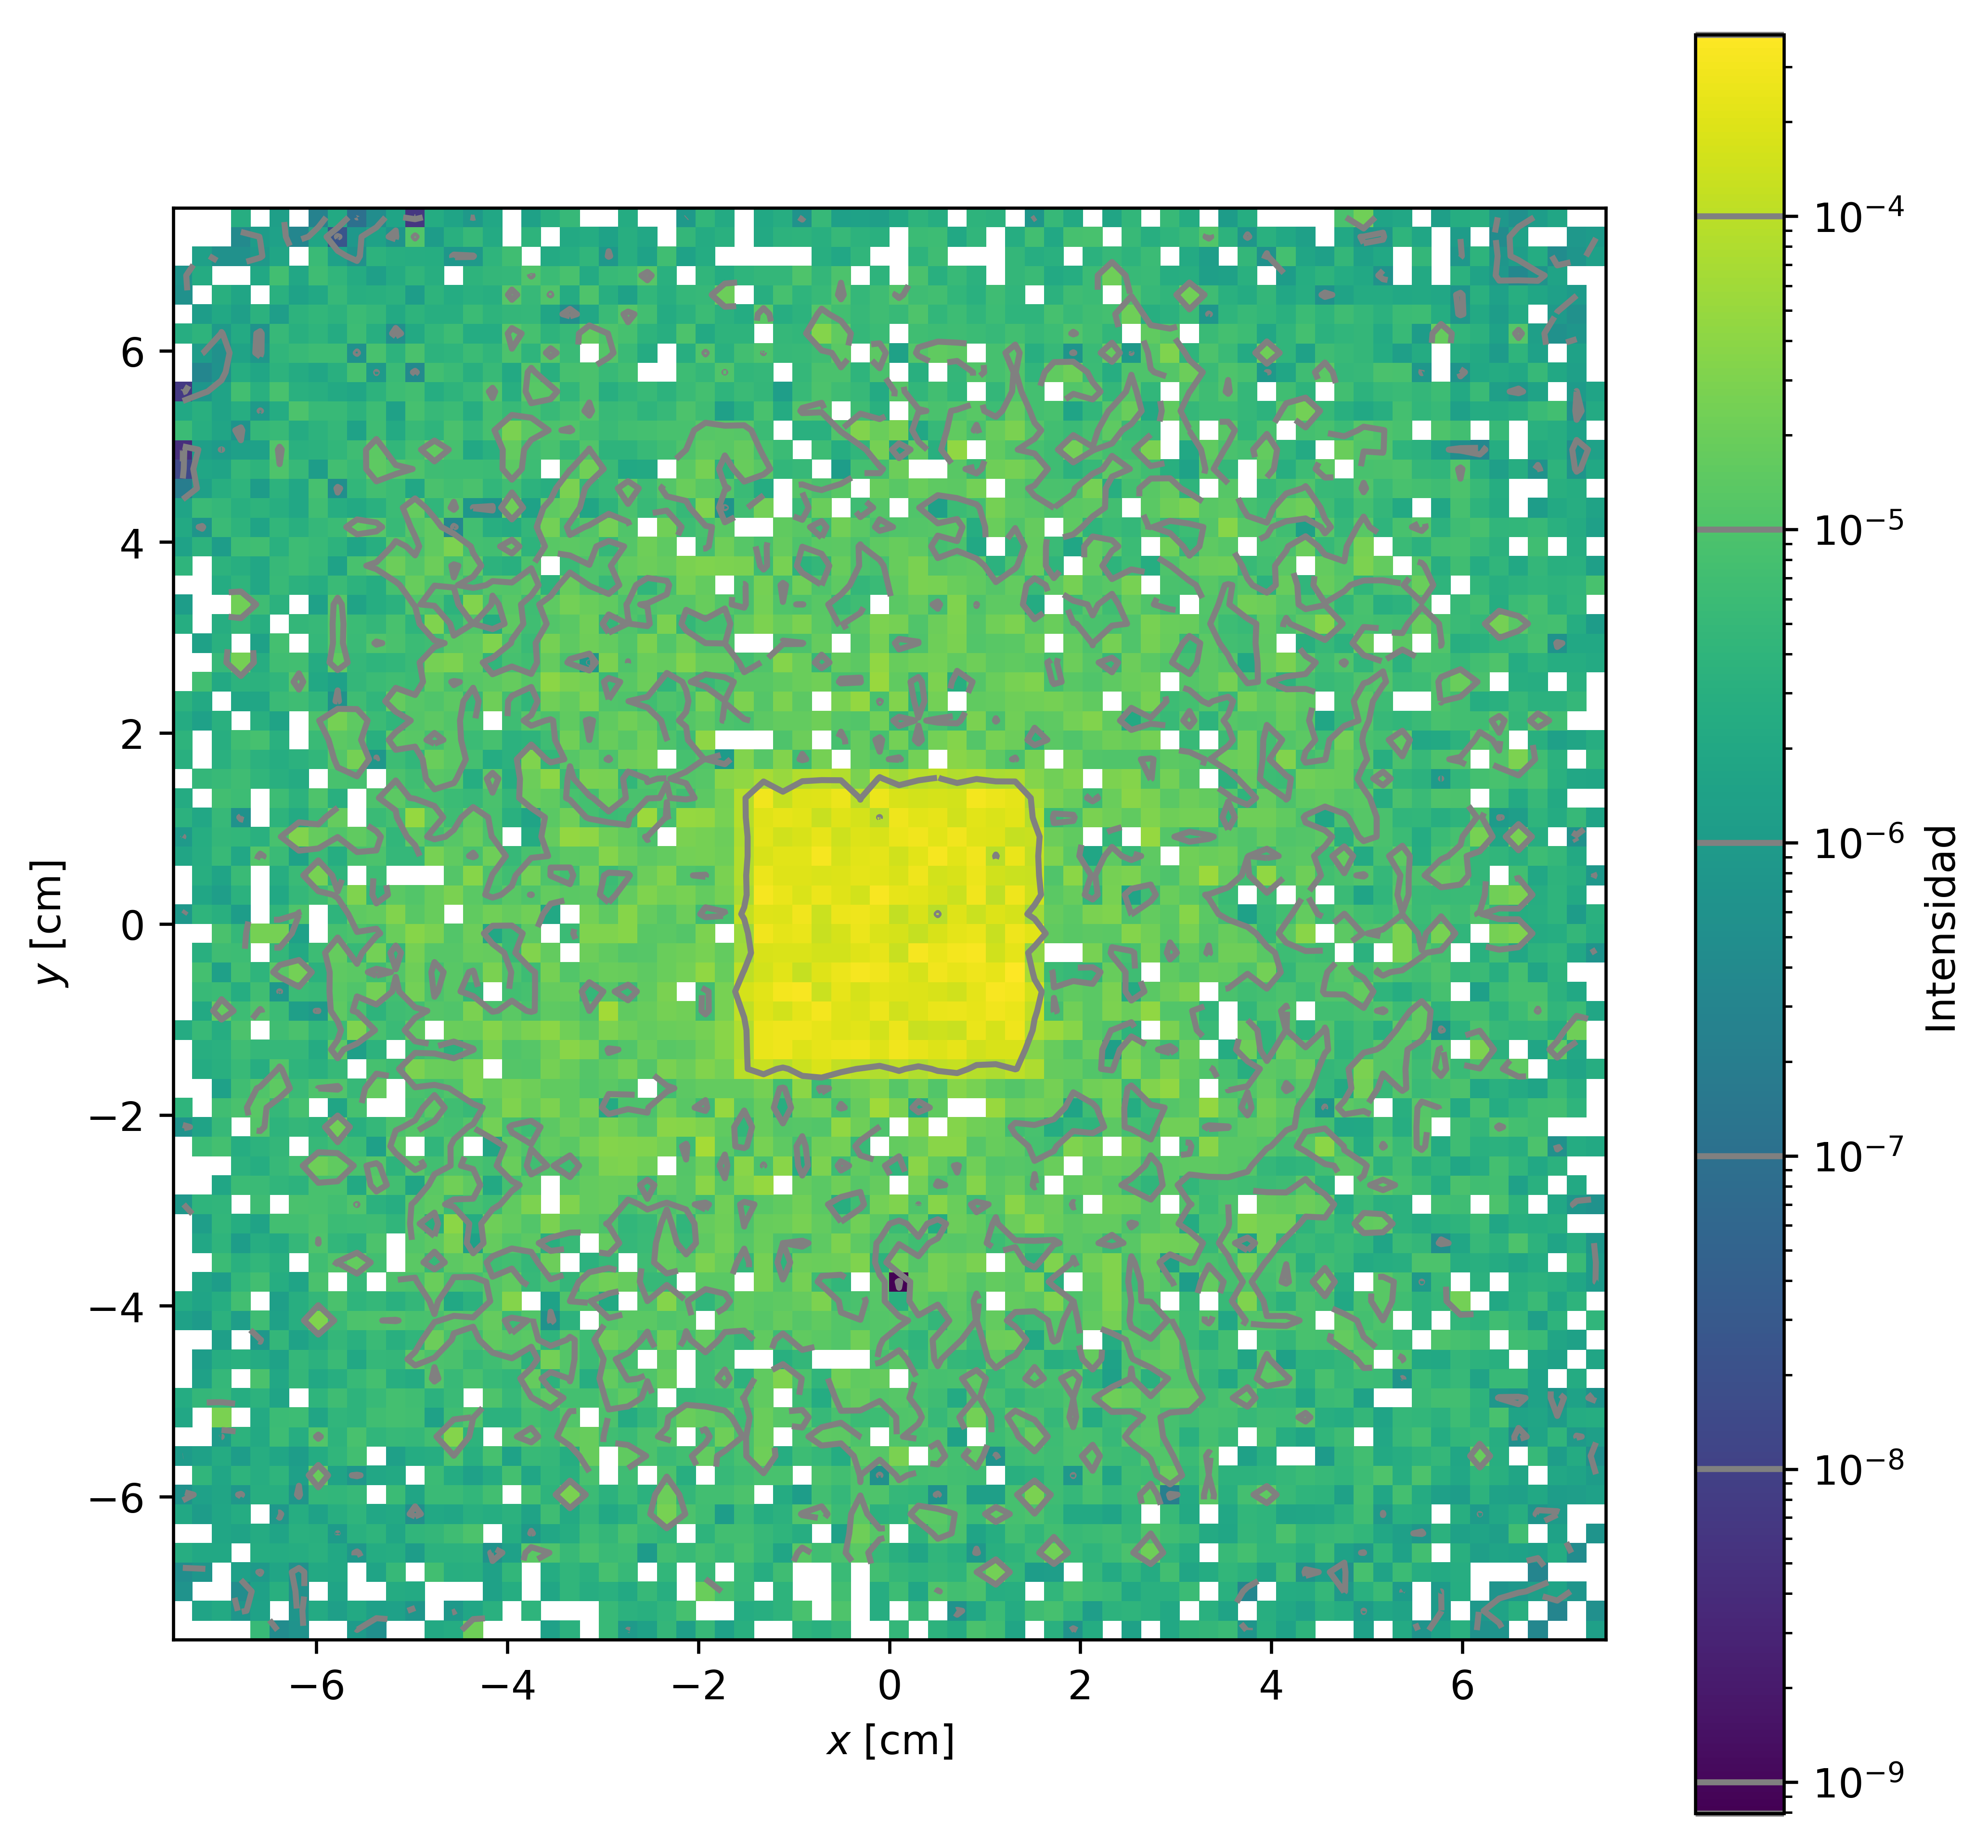
\includegraphics[width=0.75\textwidth]{figs/fig4_1.png}
    \caption{Distribuciones de $x$ vs $y$ para el \emph{trackfile} registrado en la primera corrida del tubo de vacío.}
    \label{fig:trackfile1_x_y}
\end{figure}

Este conjunto contiene dos poblaciones de neutrones claramente diferenciadas. La primera corresponde a neutrones que no han sufrido colisiones: todos ellos poseen dirección $\mu = 1$ y una letargia mínima fija, sin dispersión alguna, lo cual indica que la fuente original fue configurada con estos valores de forma determinista. La segunda población incluye neutrones que han colisionado: en este caso, las distribuciones de $\mu$ y letargia son más amplias y continuas, reflejando la dispersión introducida por las interacciones. Este comportamiento se observa en la figura \ref{fig:trackfile1_letargia_mu}, donde se presentan las distribuciones de letargia y $\mu$ para el primer trackfile. 

\begin{figure}[H]
    \centering
    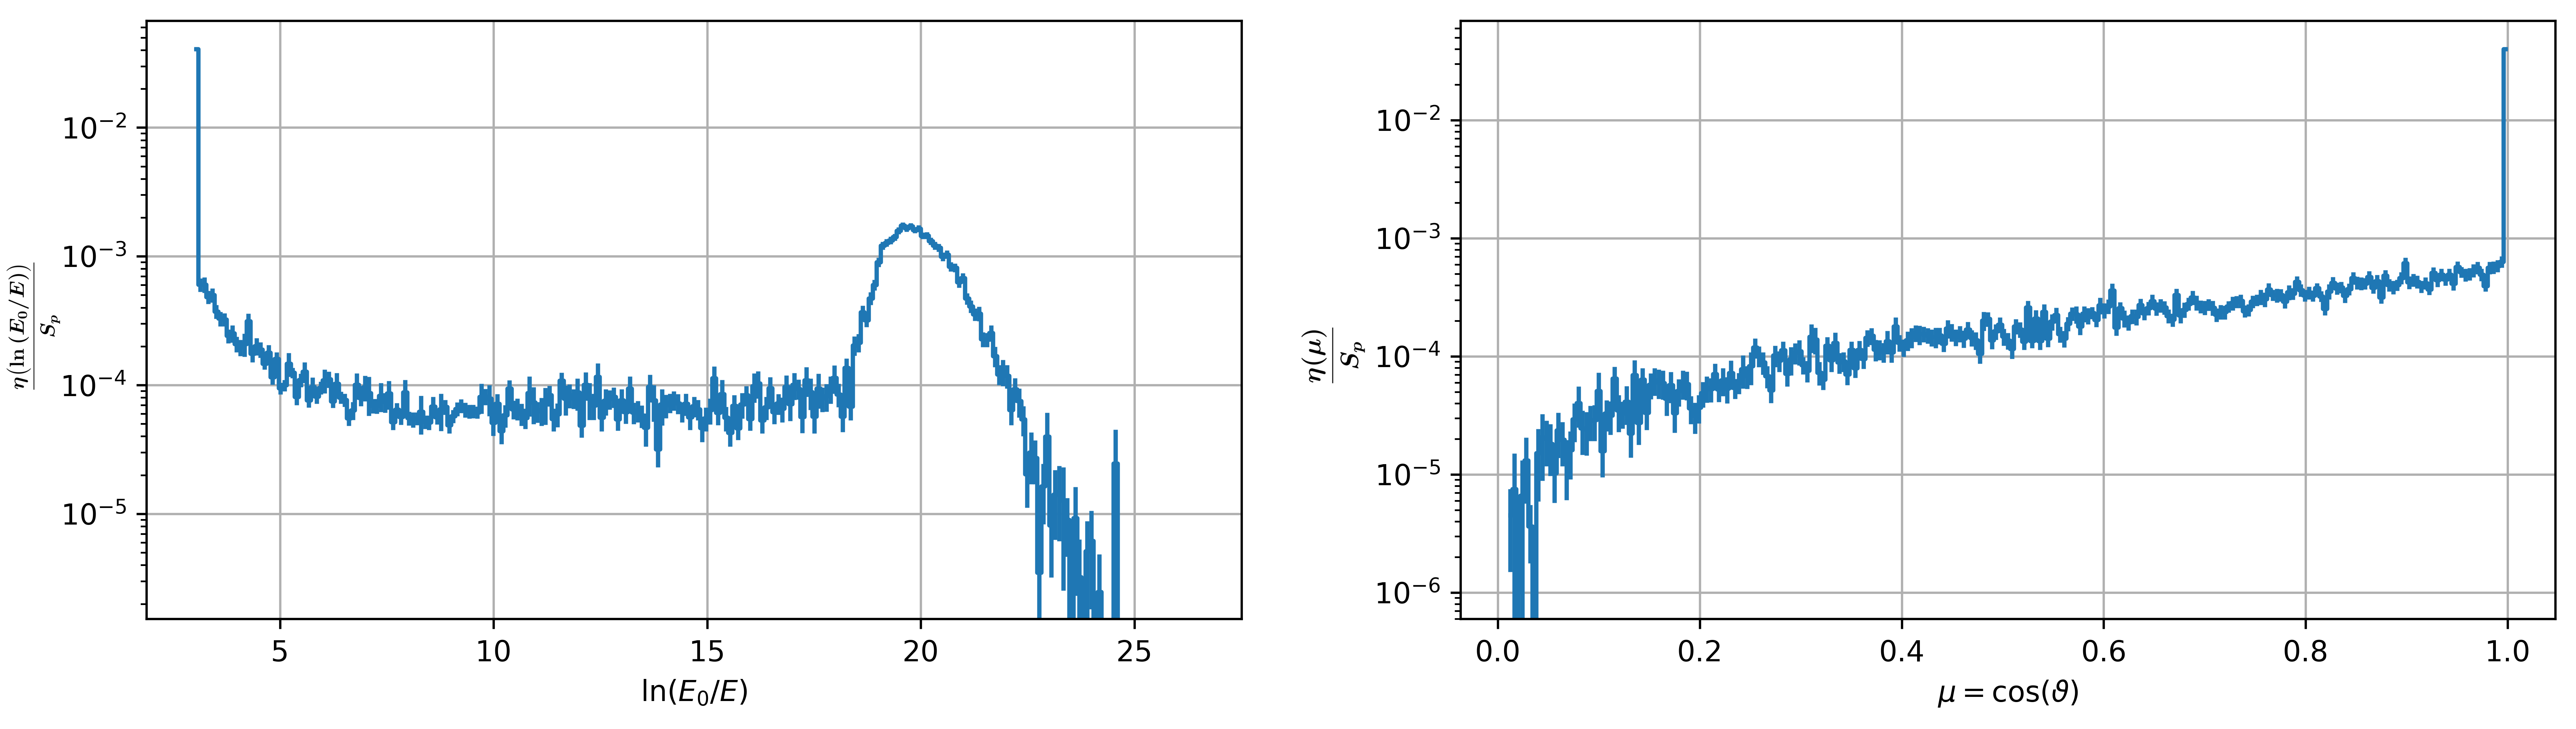
\includegraphics[width=\textwidth]{figs/fig4_2.png}
    \caption{Distribuciones de letargia y $\mu$ para el \emph{trackfile} registrado en la primera corrida del tubo de vacío, con escala logaritmica en el eje y. Se observa la presencia de dos poblaciones: una concentrada en $\mu = 1$ y letargia mínima, montada sobre una distribución continua de neutrones colisionados.}
    \label{fig:trackfile1_letargia_mu}
\end{figure}

Esta doble estructura se evidencia particularmente en los gráficos 2D de letargia vs. $\mu$, donde ambas poblaciones forman conjuntos visualmente separados (de hecho estamos hablando de dos conjuntos distintos. Repensar esto). Ver figura \ref{fig:trackfile1_letargia_mu_2}. Este fenómeno plantea un desafío para los métodos de muestreo, al requerir una representación precisa tanto de distribuciones concentradas tipo delta como de distribuciones extendidas y sus correlaciones.

\begin{figure}[H]
    \centering
    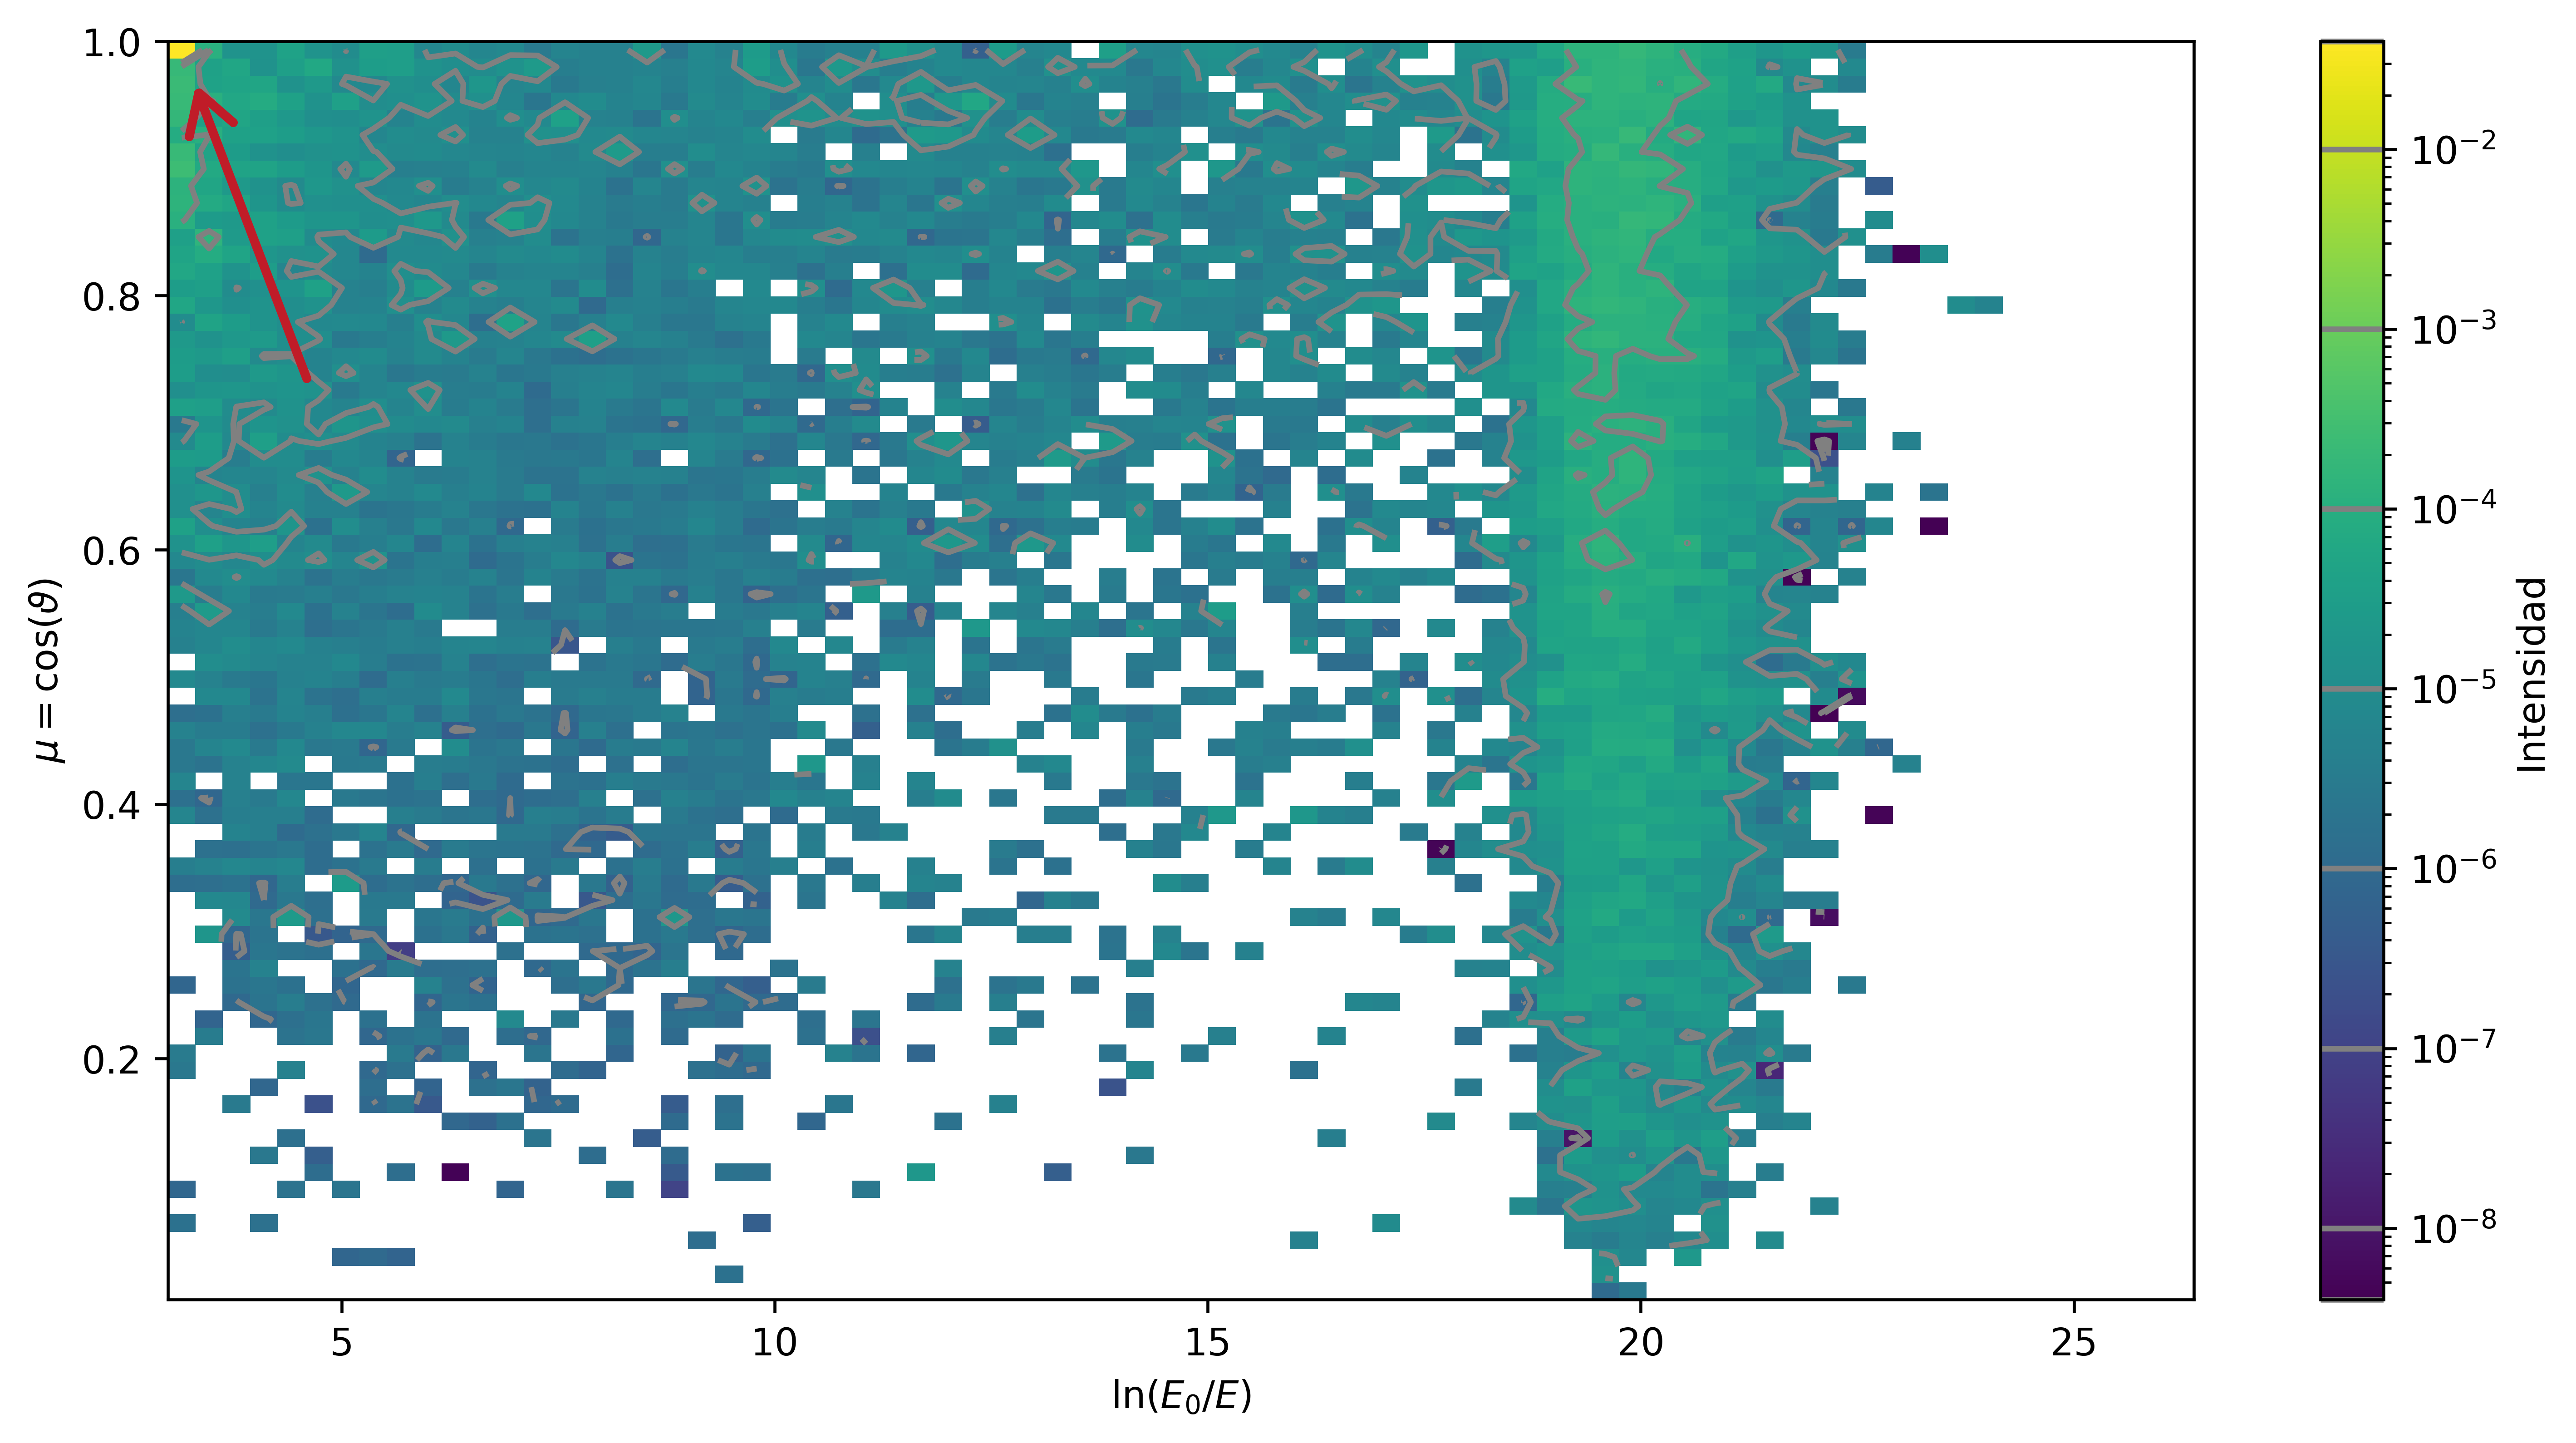
\includegraphics[width=0.9\textwidth]{figs/fig4_3.png}
    \caption{Distribuciones de letargia vs $\mu$ para el \emph{trackfile} registrado en la primera corrida del tubo de vacío. Se observa la presencia de un conjunto de neutrones graficados como un pixel en $\mu = 1$ y letargia mínima, indicando la naturaleza discreta de la fuente original. A su vez se observa la presencia de un segundo conjunto de neutrones colisionados, que se distribuyen en el plano de forma continua, con un agrupamiento sobre letargia = 20, indicando la termalización de los neutrones.}
    \label{fig:trackfile1_letargia_mu_2}
\end{figure}

A su vez se puede ver tanto en la figura \ref{fig:trackfile1_x_y} como en la figura \ref{fig:trackfile1_letargia_mu_2} que aunque el bineado del plot 2D se haya hecho con 75 bines se observa claramente que existen muchos lugares del espacio de fase donde no hay neutrones. Esto es debido a que el trackfile original tiene un número limitado de neutrones. El objetivo de este metodo propuesto consiste en poder remuestrear el trackfile original para obtener un trackfile nuevo donde se pueda observar una mejor estadística en los lugares donde el trackfile original tiene pocos neutrones. 

\subsection{Bineado uniforme de microgrupos y macrogrupos}  
Se empleó una configuración con macrogrupos y microgrupos de ancho uniforme. Se seleccionaron $n_{\text{macro}} = 6$ y $n_{\text{micro}} = 50$ para cada variable, en el orden de variables: \texttt{[ln(E0/E), x, y, mu, phi]}. Esta configuración permite evaluar el desempeño base sin ningún tipo de adaptación.

Visualmente, se observa que la distribución tipo delta en letargia mínima y $\mu = 1$ es reemplazada por un rectángulo con el ancho del bin, perdiéndose el detalle de los picos originales. El efecto del resampleo mediante bins uniformes se puede ver en las figuras \ref{fig:trackfile1_config1_letargia} y \ref{fig:trackfile1_config1_mu}, donde se comparan las distribuciones de letargia y $\mu$ entre el trackfile original y el remuestreado.

\begin{figure}[H]
    \centering
    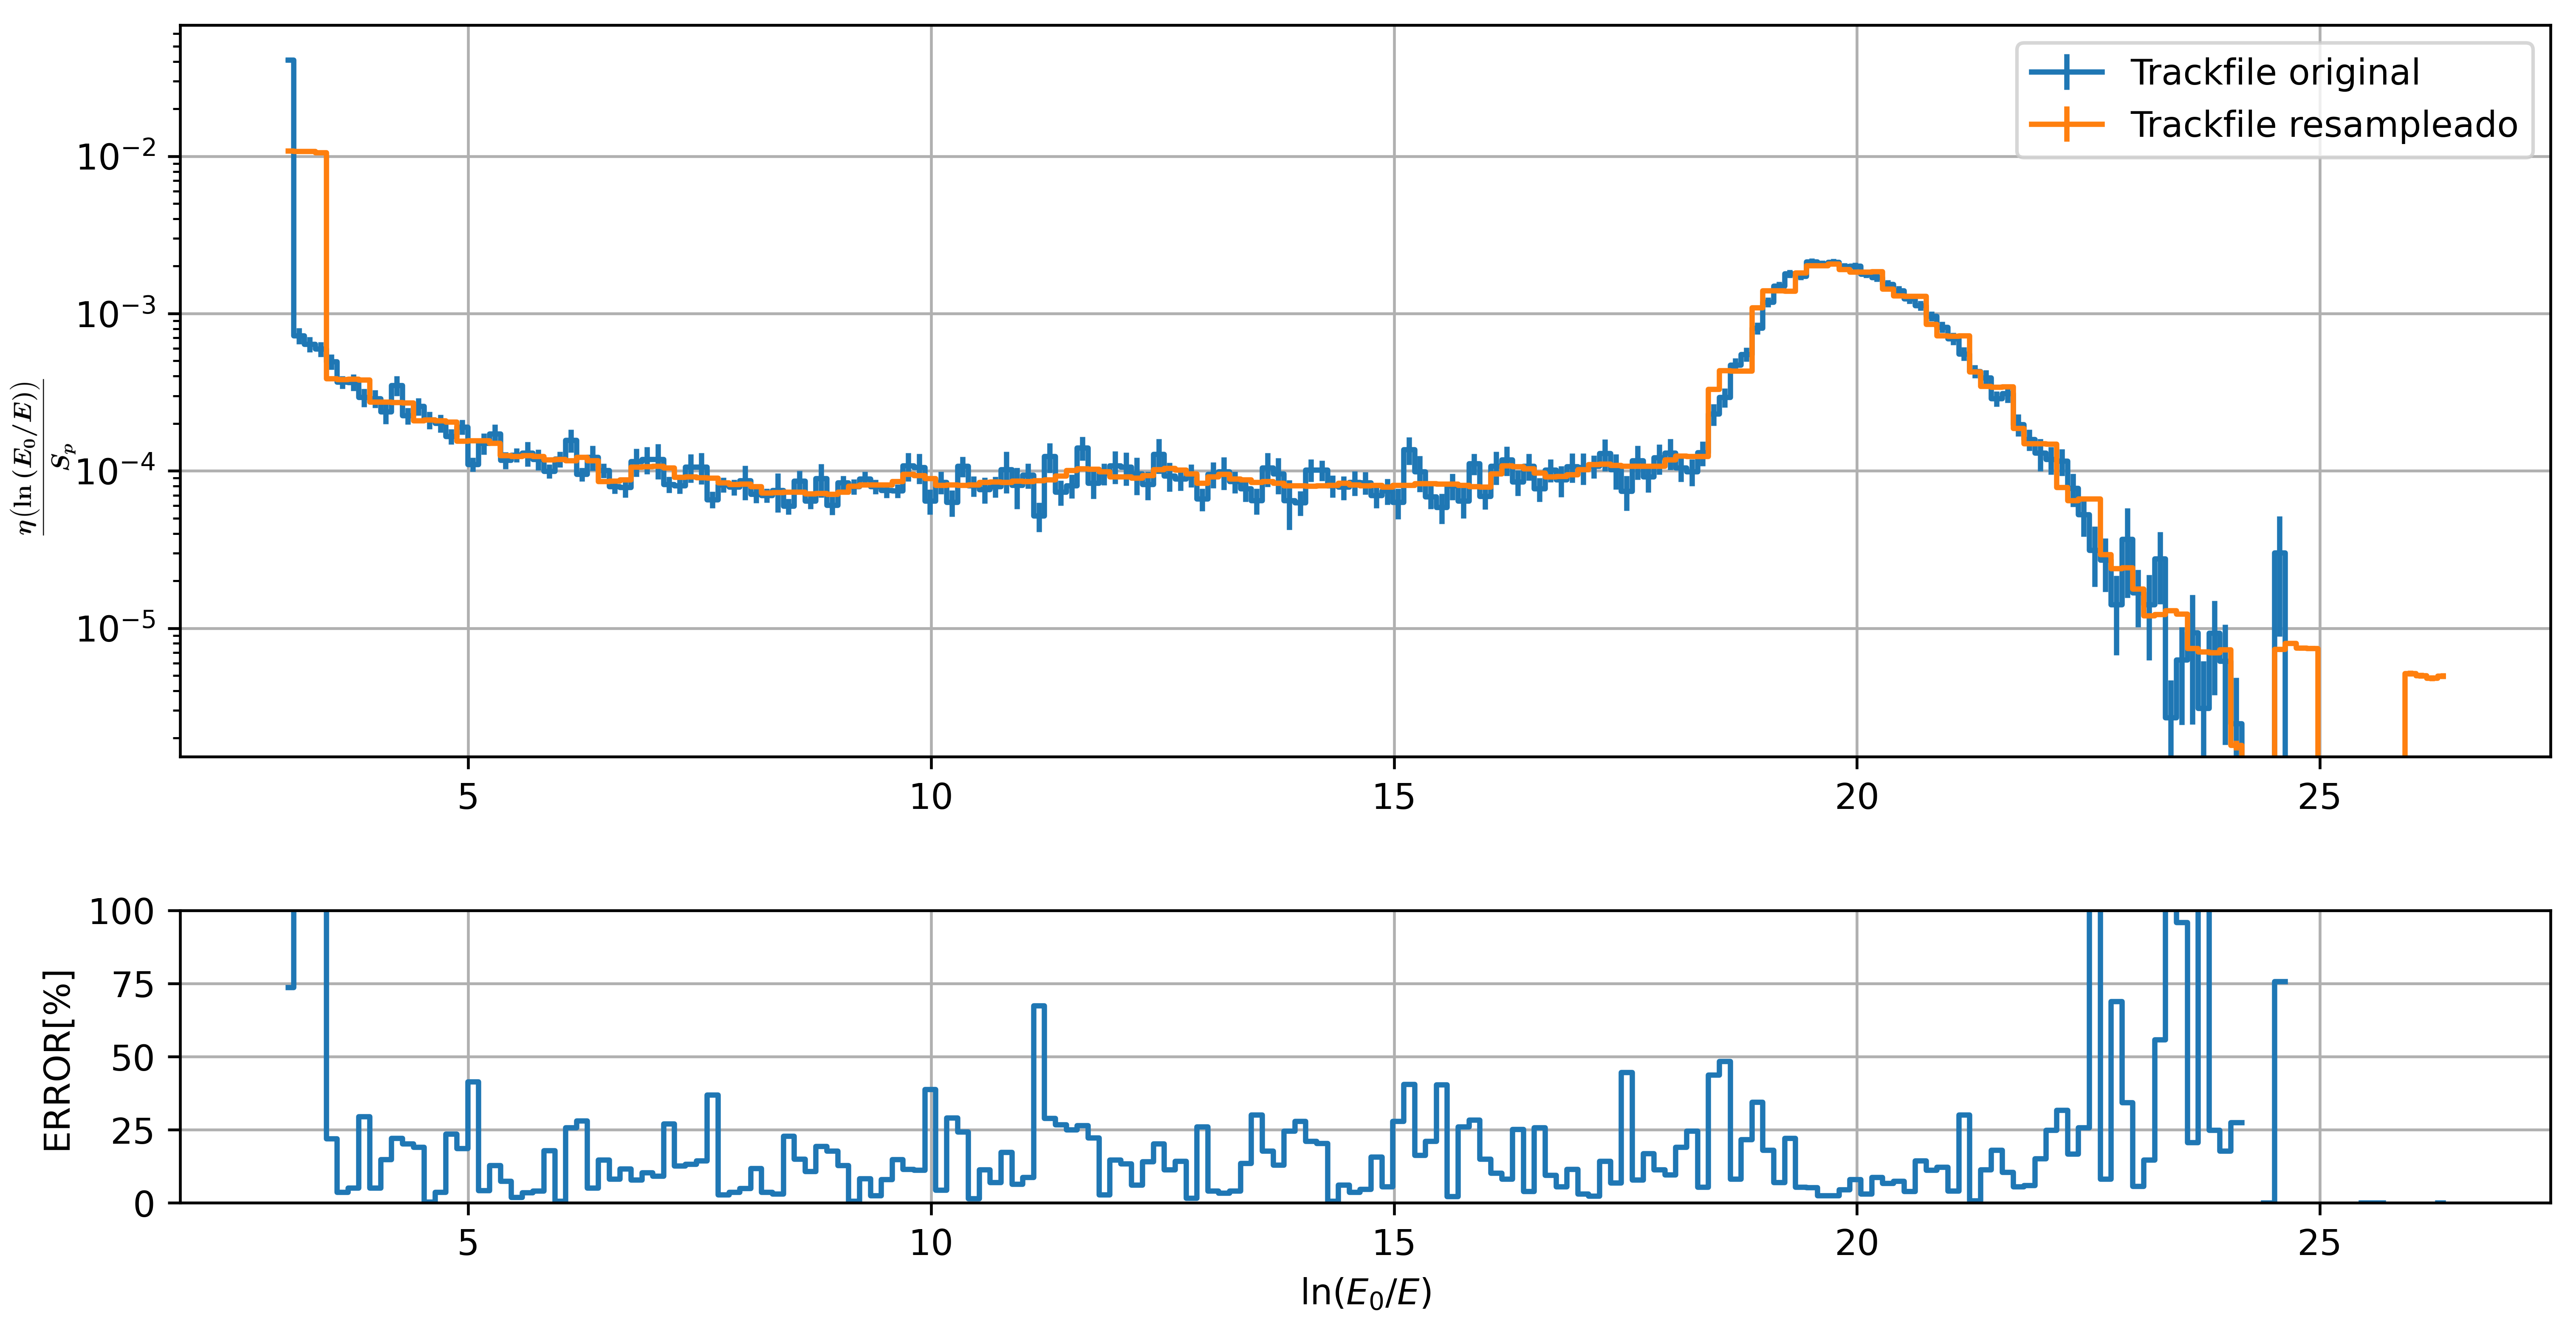
\includegraphics[width=\textwidth]{figs/fig4_4.png}
    \caption{Comparación de la distribución de letargia entre el trackfile original y el trackfile remuestreado. Se observa el efecto de la discretización uniforme en la distribución de letargia.}
    \label{fig:trackfile1_config1_letargia}
\end{figure}

\begin{figure}[H]
    \centering
    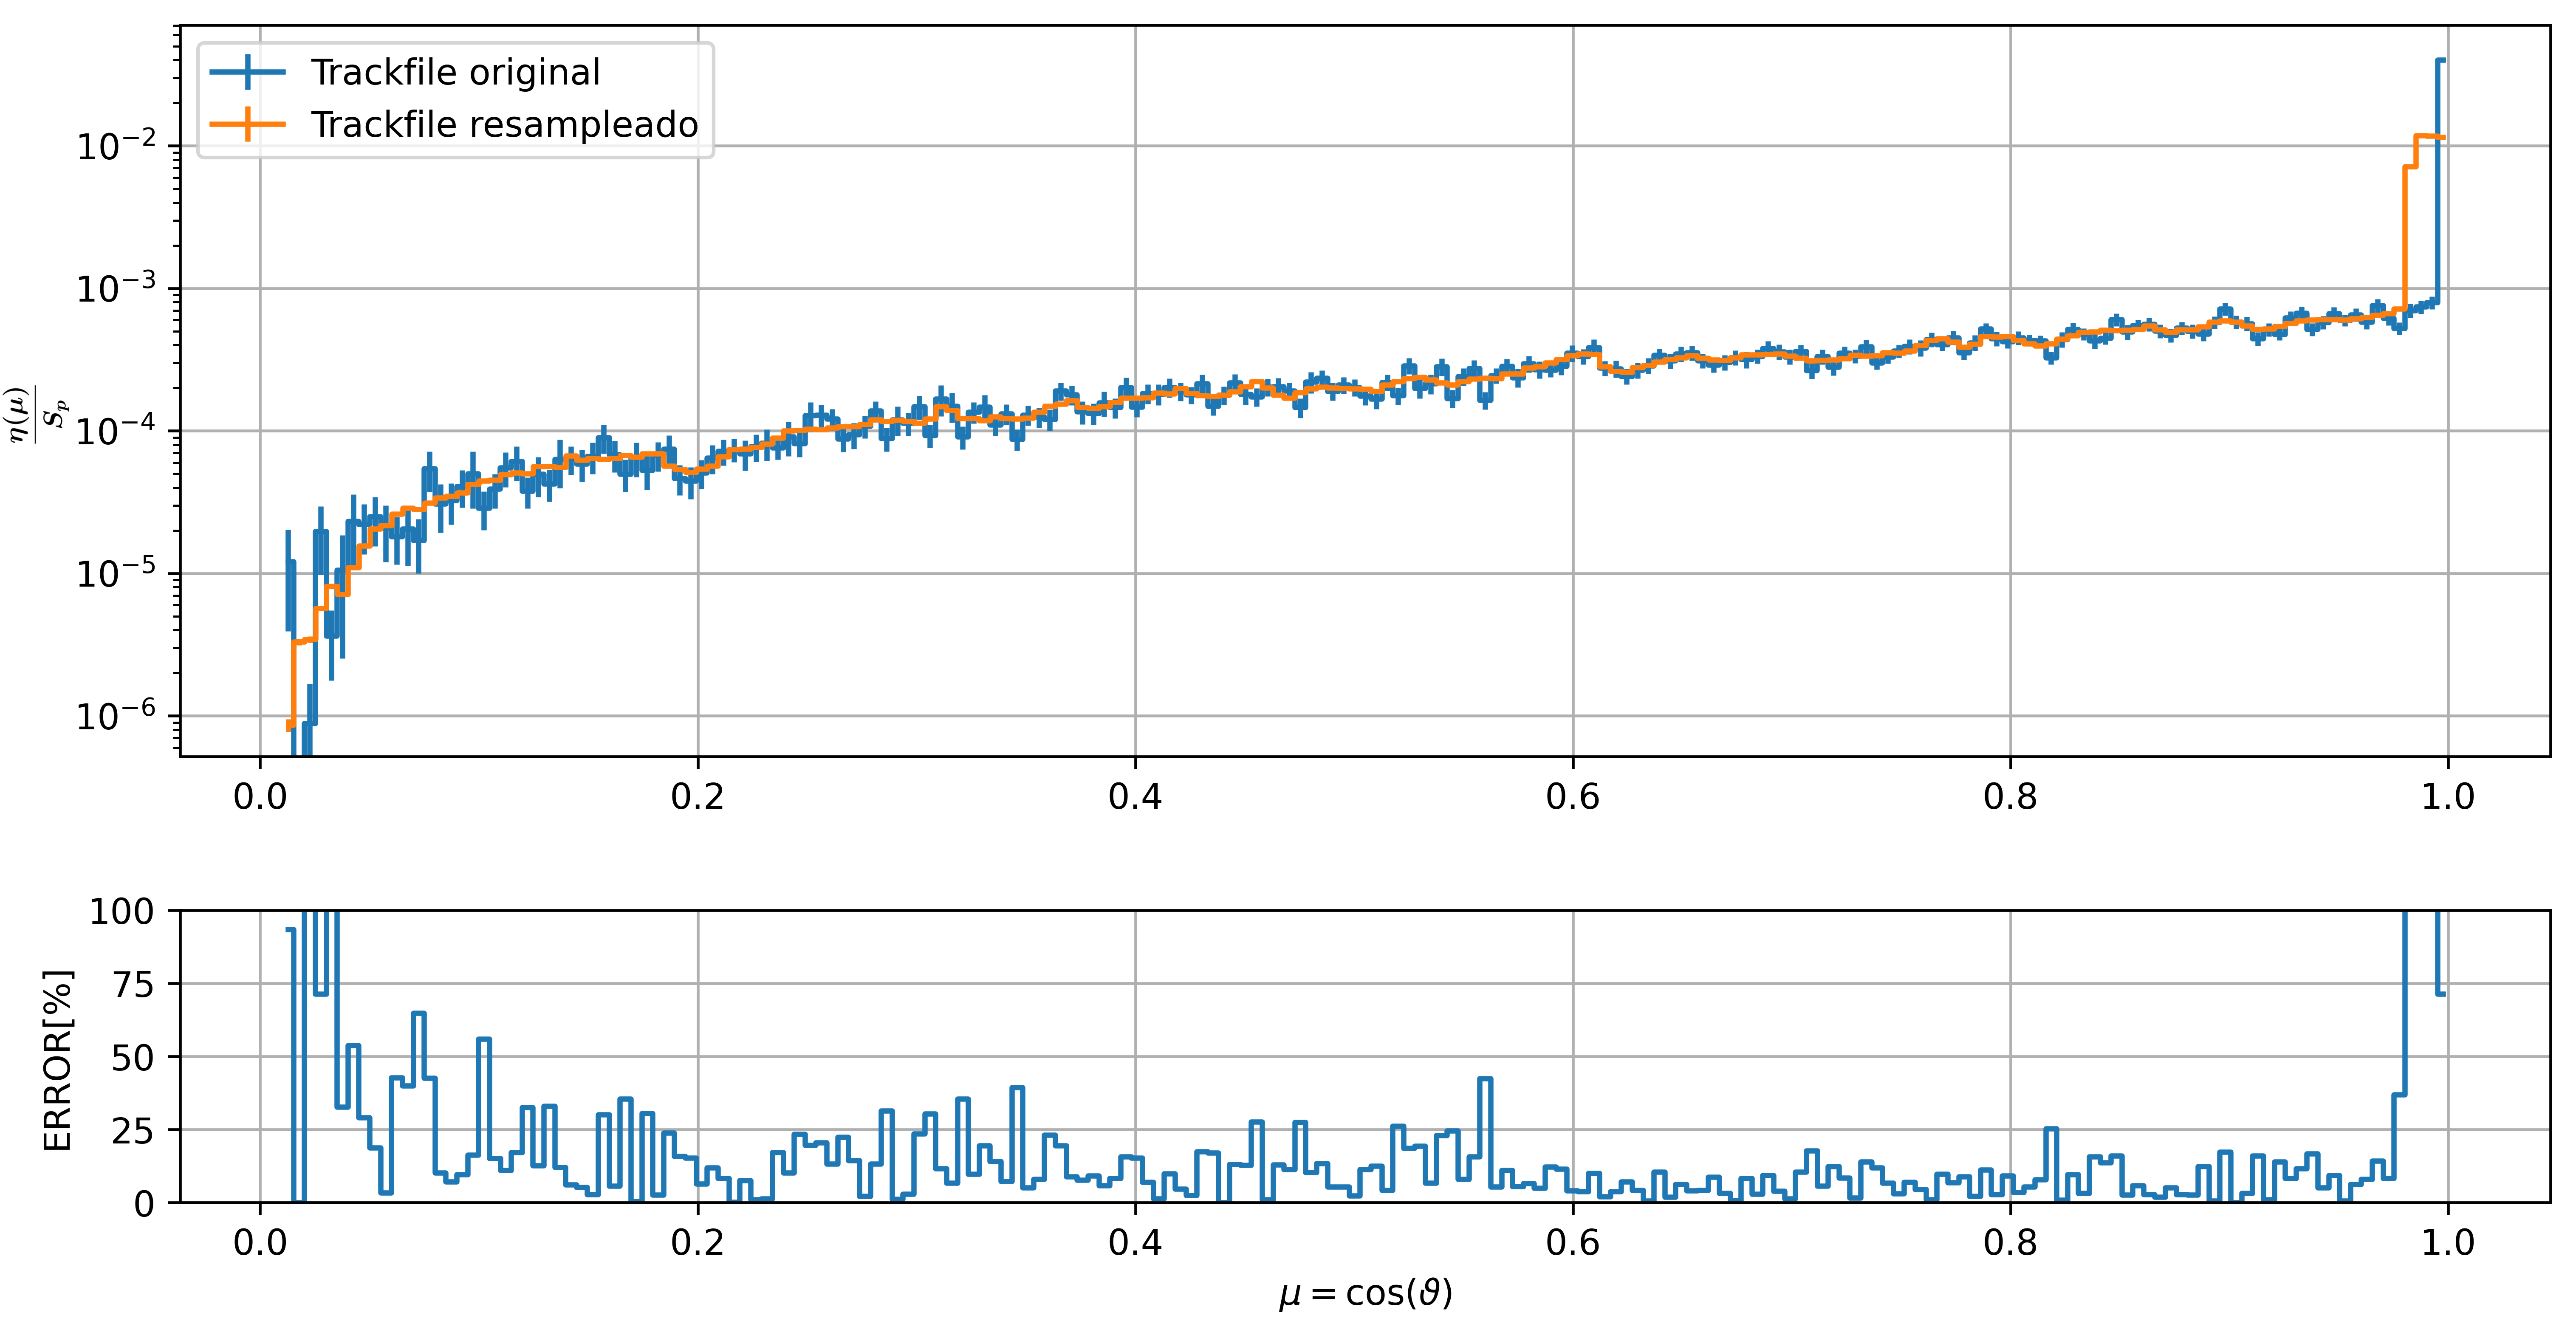
\includegraphics[width=\textwidth]{figs/fig4_5.png}
    \caption{Comparación de la distribución de $\mu$ entre el trackfile original y el trackfile remuestreado. Se observa el efecto de la discretización uniforme en la distribución de $\mu$.}
    \label{fig:trackfile1_config1_mu}
\end{figure}

Este efecto captado en las figuras \ref{fig:trackfile1_config1_letargia} y \ref{fig:trackfile1_config1_mu} produce que los neutrones que originalmente viajaban por el vacio perfectamente colimados y monoenergeticos ahora se descolimen y obtengan variacion en energia. Esto produce que los neutrones que viajaban cerca de la interfaz agua vacio ahora puedan ingresar al agua. Esto produce una perdida en la corriente por el vacio y una ganancia en la corriente por el agua. 

Otro efecto que se observa es que la resolucion de los histogramas, al ser de bineado uniforme, no permite atribuir mas bines donde haya mas estadistica. Por lo tanto no se asignan mas bines a las deltas de mu y letargia, ni se asignan mas bines a la zona de termalizacion en la letargia.

% Además, en las distribuciones espaciales, tanto $x$ como $y$, se elimina el ruido estadístico original de forma local pero sin suavizado general, reflejando el bineado uniforme. Esto se observa en la figura \ref{fig:trackfile1_config1_x}, donde se comparan las distribuciones de $x$ entre el trackfile original y el remuestreado. 

% \begin{figure}[h]
%     \centering
%     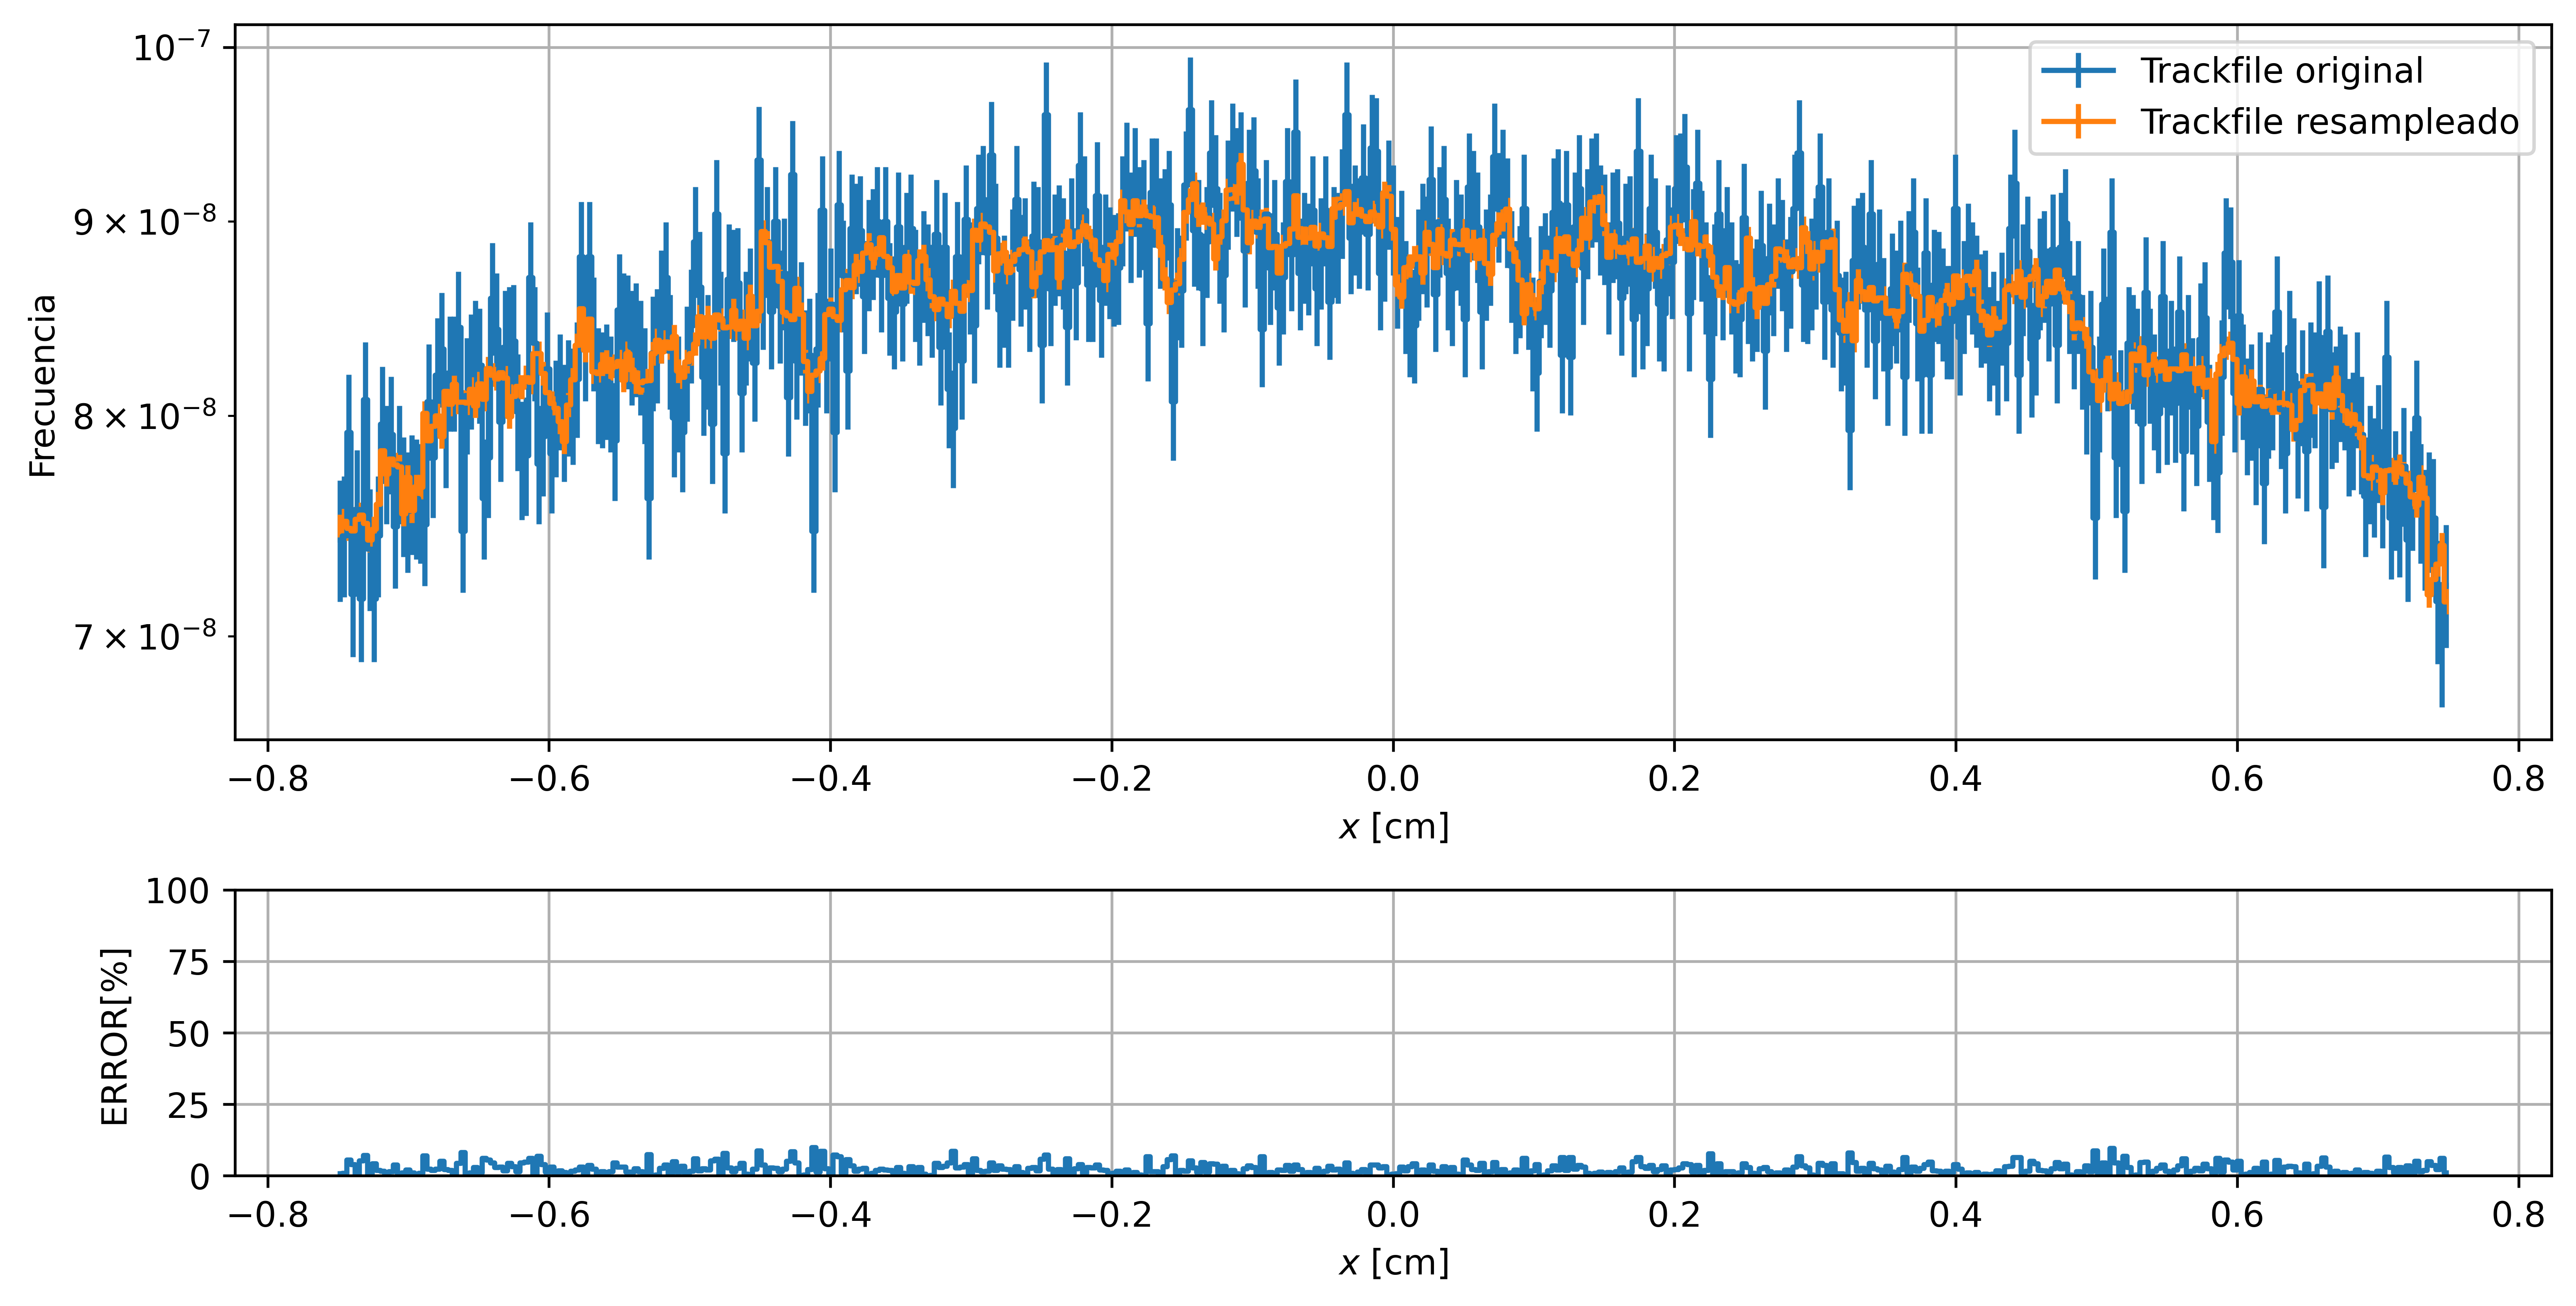
\includegraphics[width=\textwidth]{figs/fig2_6.png}
%     \caption{Comparacion de la distribucion de x entre el trackfile original y el trackfile remuestreado. Se observa el efecto de la discretizacion uniforme en la distribucion de x debido a que se reduce el ruido a nivel local pero se observa el bineado uniforme.}
%     \label{fig:trackfile1_config1_x}
% \end{figure}

Analizando el caso del ploteo 2D de x vs y se observa el efecto del bineado uniforme en los macrogrupos debido a que se observa que el resampleo deforma la distribucion original. En la figura \ref{fig:trackfile1_x_y} se observa el canal de vacio y alrededor la estadistica del agua, de forma uniforme alrededor del canal. Sin embargo en la figura \ref{fig:trackfile1_x_y_uniforme} se observa que se difumina parte de la estadistica del canal de vacio dentro del agua en forma de cruz. Esto se debe a que hay macrogrupos que intersectan el canal de vacio y el agua y produce que los neutrones que viajaban cerca de la interfaz agua vacio ahora puedan aparecer en el agua.

\begin{figure}[H]
    \centering
    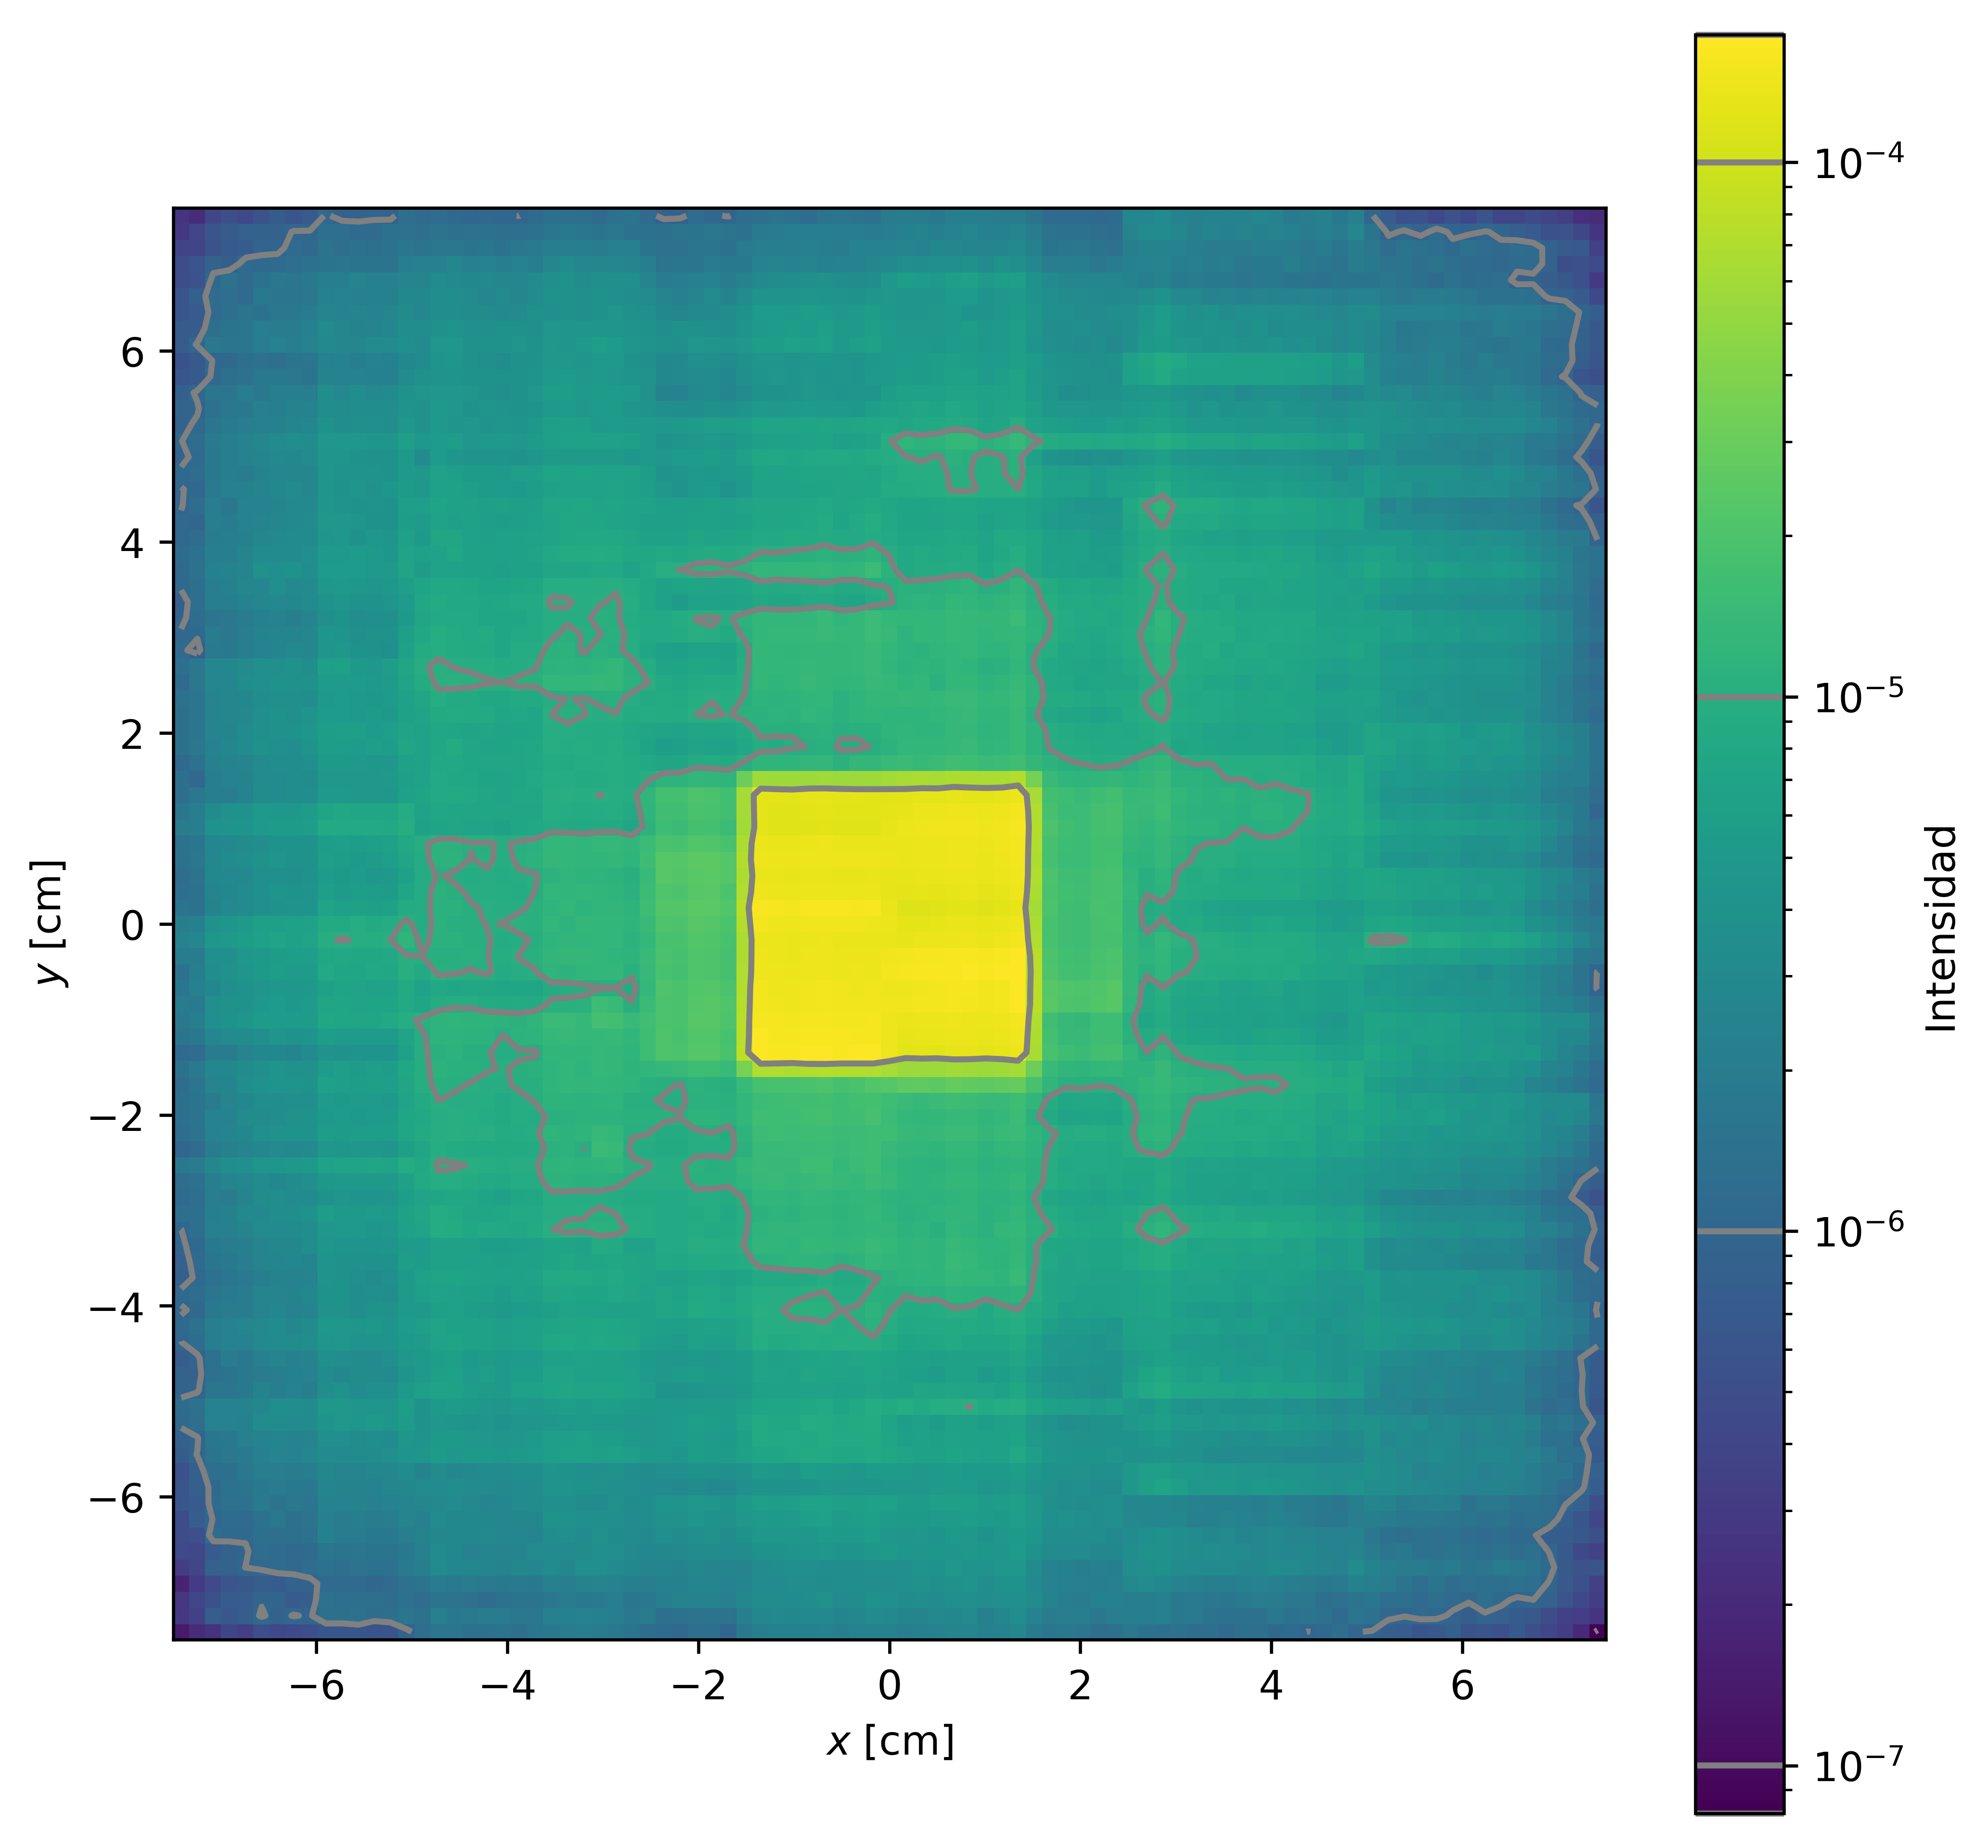
\includegraphics[width=0.75\textwidth]{figs/fig4_6.png}
    \caption{Distribuciones de $x$ vs $y$ para el \emph{trackfile} remuestreado utilizando discretizacion uniforme tanto para macrogrupos como para microgrupos.}
    \label{fig:trackfile1_x_y_uniforme}
\end{figure}

En la tabla \ref{tab:KL_parciales_equal_columns} se presentan las divergencias KL 1D y 2D, tanto de forma parcial como total, para la configuración de bineado uniforme. Estos valores no indican informacion utilizable para decidir si el muestreo es aceptable o no. Sin embargo es util a modo de comparacion contra otros bineados que posteriormente se van a mostrar. 

\begin{table}[H]
    \centering
    \caption{Divergencia KL parcial y total para la configuración \texttt{Equal / Equal}.}
    \label{tab:KL_parciales_equal_columns}
    \begin{tabular}{ll@{\hspace{2cm}}ll}
    \toprule
    \multicolumn{2}{c}{\textbf{KL 1D}} & \multicolumn{2}{c}{\textbf{KL 2D}} \\
    \cmidrule(lr){1-2} \cmidrule(lr){3-4}
    \textbf{Parámetro} & \textbf{Valor} & \textbf{Parámetros} & \textbf{Valor} \\
    \midrule
    $\ln(E_0/E)$ & 6.0372e-01 & $\ln(E_0/E), x$ & 4.3450e+00 \\
    $x$ & 3.3379e-01 & $\ln(E_0/E), y$ & 4.3407e+00 \\
    $y$ & 3.3882e-01 & $\ln(E_0/E), \mu$ & 1.2565e+01 \\
    $\mu$ & 1.3727e+01 & $\ln(E_0/E), \phi$ & 4.4713e+00 \\
    $\phi$ & 4.5827e-01 & $x, y$ & 2.3899e+00 \\
    & & $x, \mu$ & 1.1431e+01 \\
    & & $x, \phi$ & 2.1703e+00 \\
    & & $y, \mu$ & 1.1432e+01 \\
    & & $y, \phi$ & 2.1283e+00 \\
    & & $\mu, \phi$ & 1.1552e+01 \\
    \midrule
    \textbf{Suma KL 1D} & \textbf{1.5462e+01} & \textbf{Suma KL 2D} & \textbf{6.6825e+01} \\
    \bottomrule
    \end{tabular}
    \vspace{0.5em}
    
    KL total = 8.2286e+01
\end{table}

\subsection{Bineado uniforme de microgrupos y macrogrupos con bordes manuales}

Para mitigar la pérdida de información debido a los problemas de resolucion del bineado uniforme, se incorporó la posibilidad de definir manualmente los bordes de los macrogrupos y microgrupos en las variables. Esto permitió aislar tanto la región correspondiente al canal de vacío, evitando que neutrones colimados se mezclen con partículas moderadas, como los neutrones de letargia mínima y $\mu = 1$.

% Se analizaron tres configuraciones diferentes:

% \begin{itemize}
%     \item \textbf{Caso A}: definición manual en las variables $x$ e $y$, asignando los bordes de x = -1.5 cm y x = 1.5 cm, y de y = -1.5 cm y y = 1.5 cm. 
%     \item \textbf{Caso B}: definición manual en letargia y $\mu$, asignando los bordes de letargia = minima + 1e-9, y de $\mu = 1 - 1e-9$.
%     \item \textbf{Caso C}: definición manual en las cuatro variables ($x$, $y$, $\mu$, letargia).
% \end{itemize}

Se definieron bordes manuales para las cuatro variables principales con el objetivo de aislar las regiones de mayor interés físico y evitar la mezcla entre poblaciones distintas. Los bordes se establecieron de la siguiente manera:

\begin{itemize}
    \item \textbf{Letargia:} se fijó un borde en el valor mínimo de letargia + 1e-9 (correspondiente a los neutrones no colisionados) y el resto de los bordes se distribuyeron uniformemente en el rango restante.
    \item \textbf{$\mu$:} se colocó un borde en $\mu = 1-1e-9$ (dirección perfectamente colimada), separando así los neutrones no dispersados del resto; los demás bordes se ubicaron de forma uniforme en el intervalo restante.
    \item \textbf{$x$ e $y$:} se asignaron bordes en las posiciones que delimitan el canal de vacío ($x = \pm 1.5\,\text{cm}$ y $y = \pm 1.5\,\text{cm}$), de modo que los macrogrupos coincidan con la geometría del canal y el agua circundante. El resto de los bordes se distribuyeron uniformemente fuera de esa región.
\end{itemize}

Esta segmentación permite preservar la física del sistema y mejorar la representación de las poblaciones diferenciadas en el proceso de remuestreo.

Al procesar el \emph{trackfile} original con esta configuración, se observa que la distribución de letargia y $\mu$ se mantiene más cercana a la original, aunque aún se presenta un efecto debido a la falta de resolucion donde hay mas estadistica. En la figura \ref{fig:trackfile1_config1_letargia_manual} se observa que la distribucion remuestrada conserva la delta en letargia minima. Sin embargo seria mejor obtener mas bines en la zona de letargia minima y en la zona de termalizacion. En la figura \ref{fig:trackfile1_config1_mu_manual} se observa que la distribucion remuestrada conserva la delta en $\mu = 1$. Sin embargo seria mejor obtener mas bines en la zona de $\mu = 1$ y menos donde hay menos estadistica.

\begin{figure}[H]
    \centering
    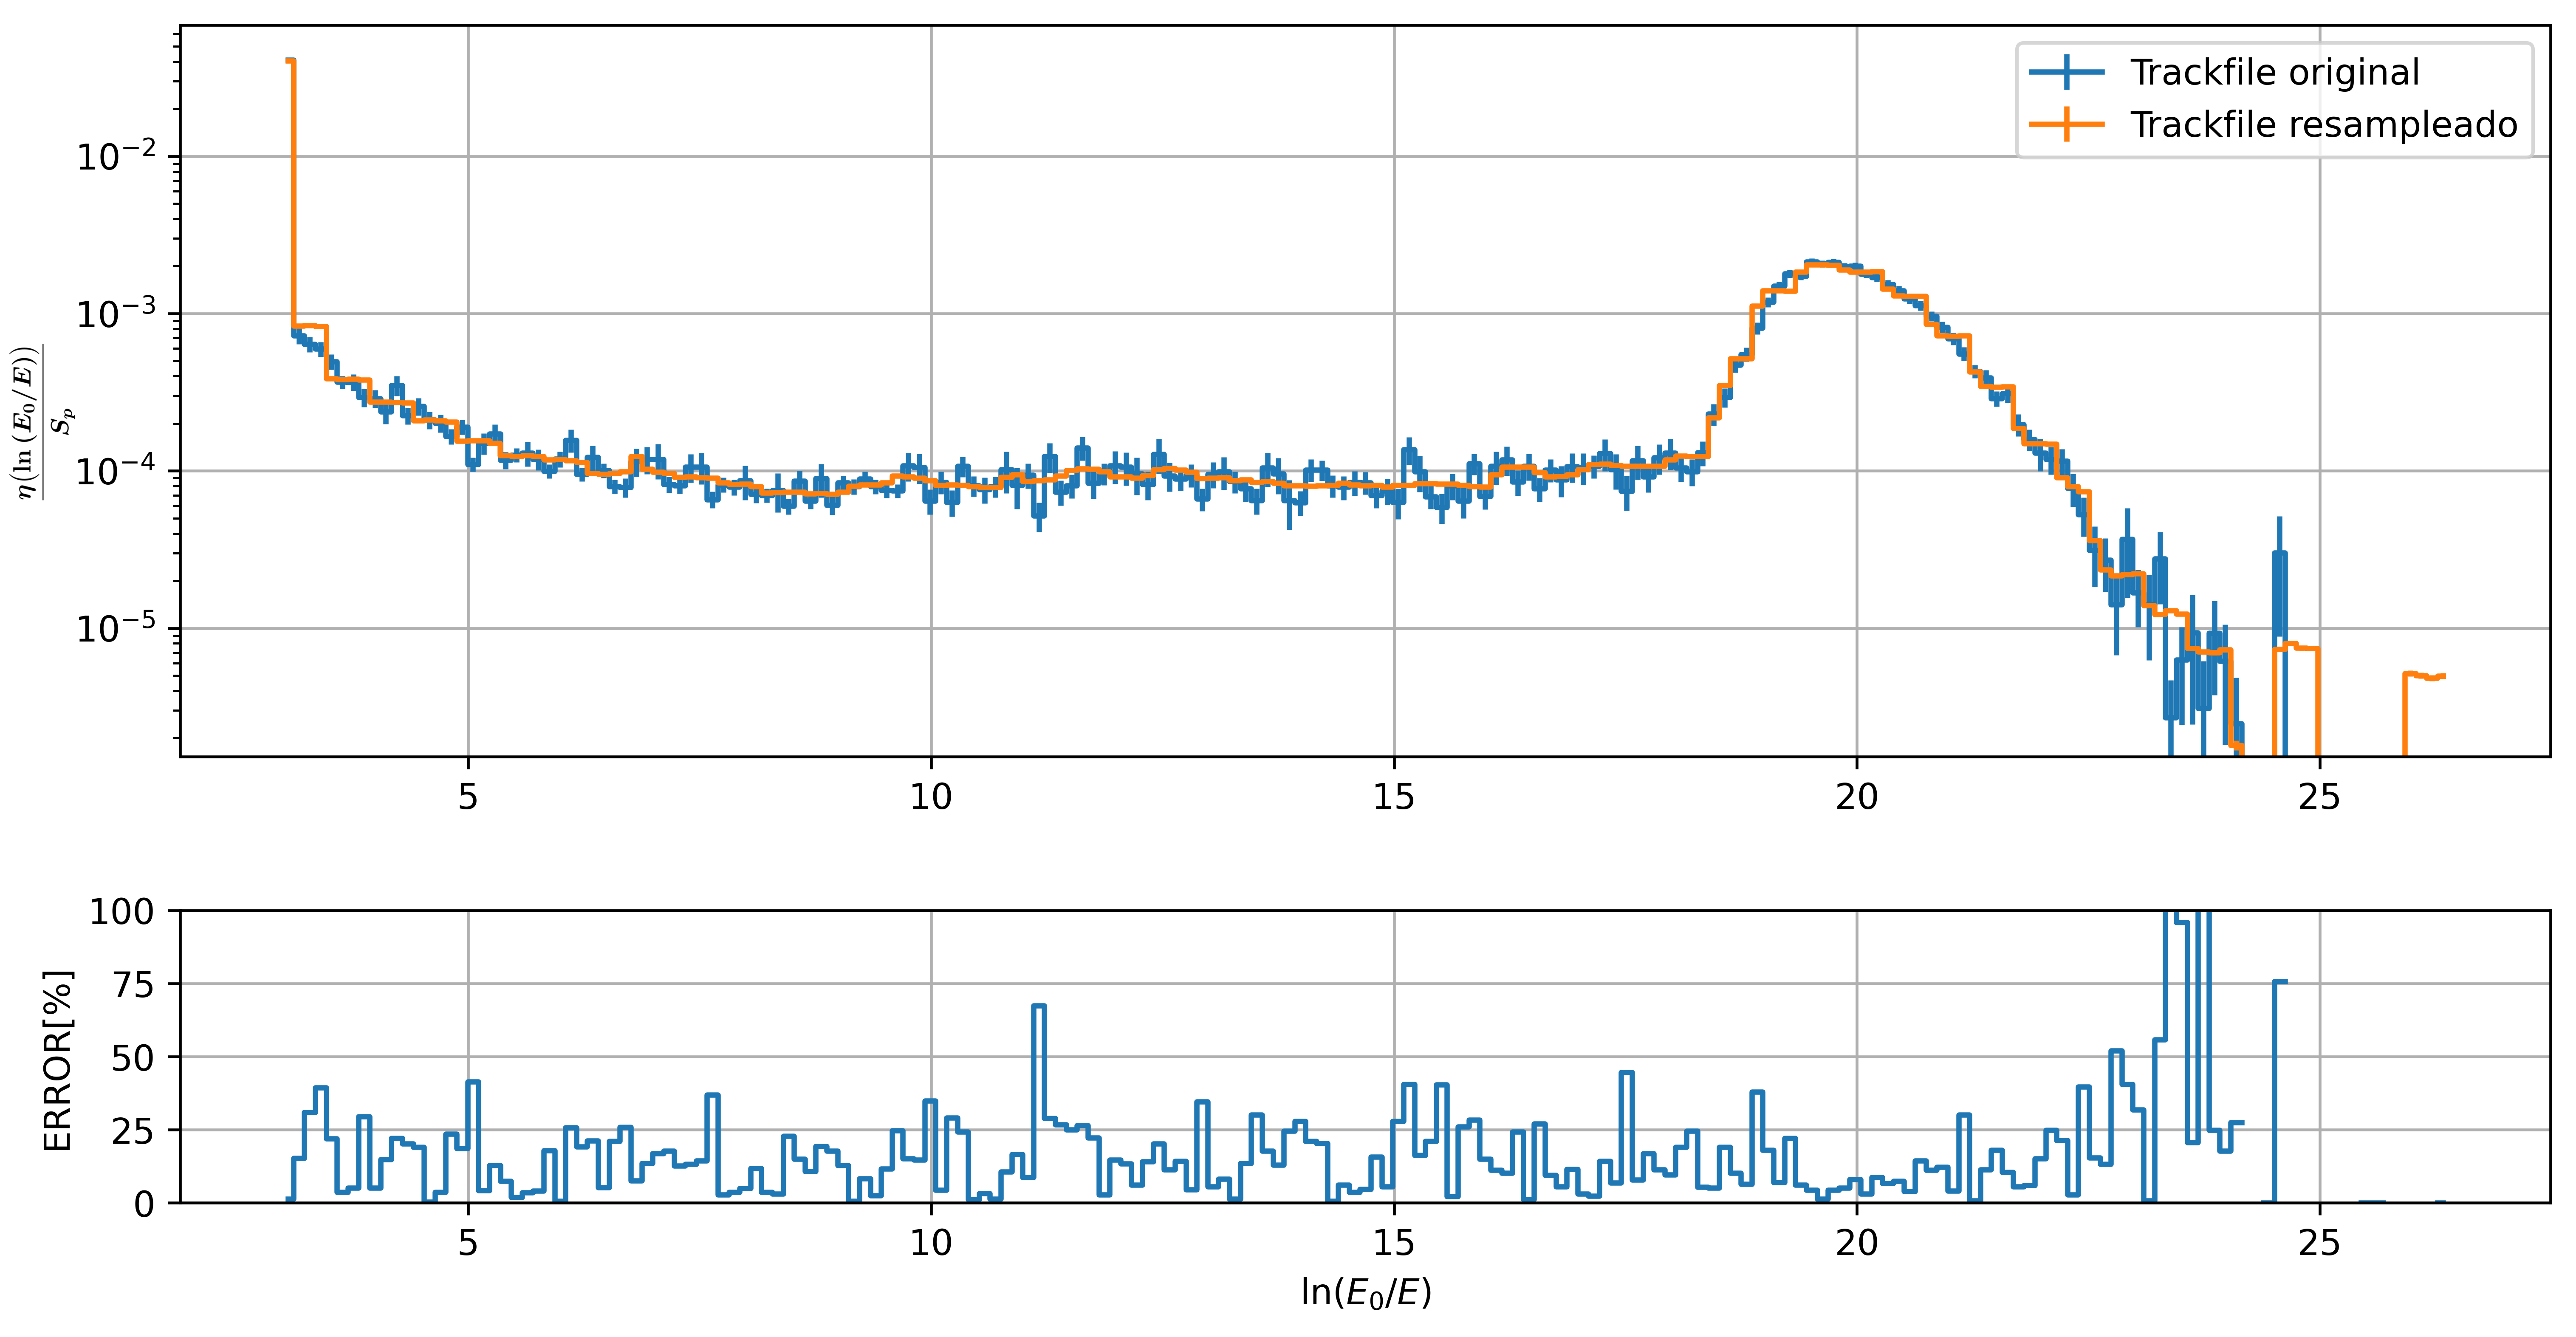
\includegraphics[width=\textwidth]{figs/fig4_7.png}
    \caption{Comparación de la distribución de letargia entre el trackfile original y el trackfile remuestreado. Se observa el efecto de separar manualmente los neutrones con letargia minima.}
    \label{fig:trackfile1_config1_letargia_manual}
\end{figure}

\begin{figure}[H]
    \centering
    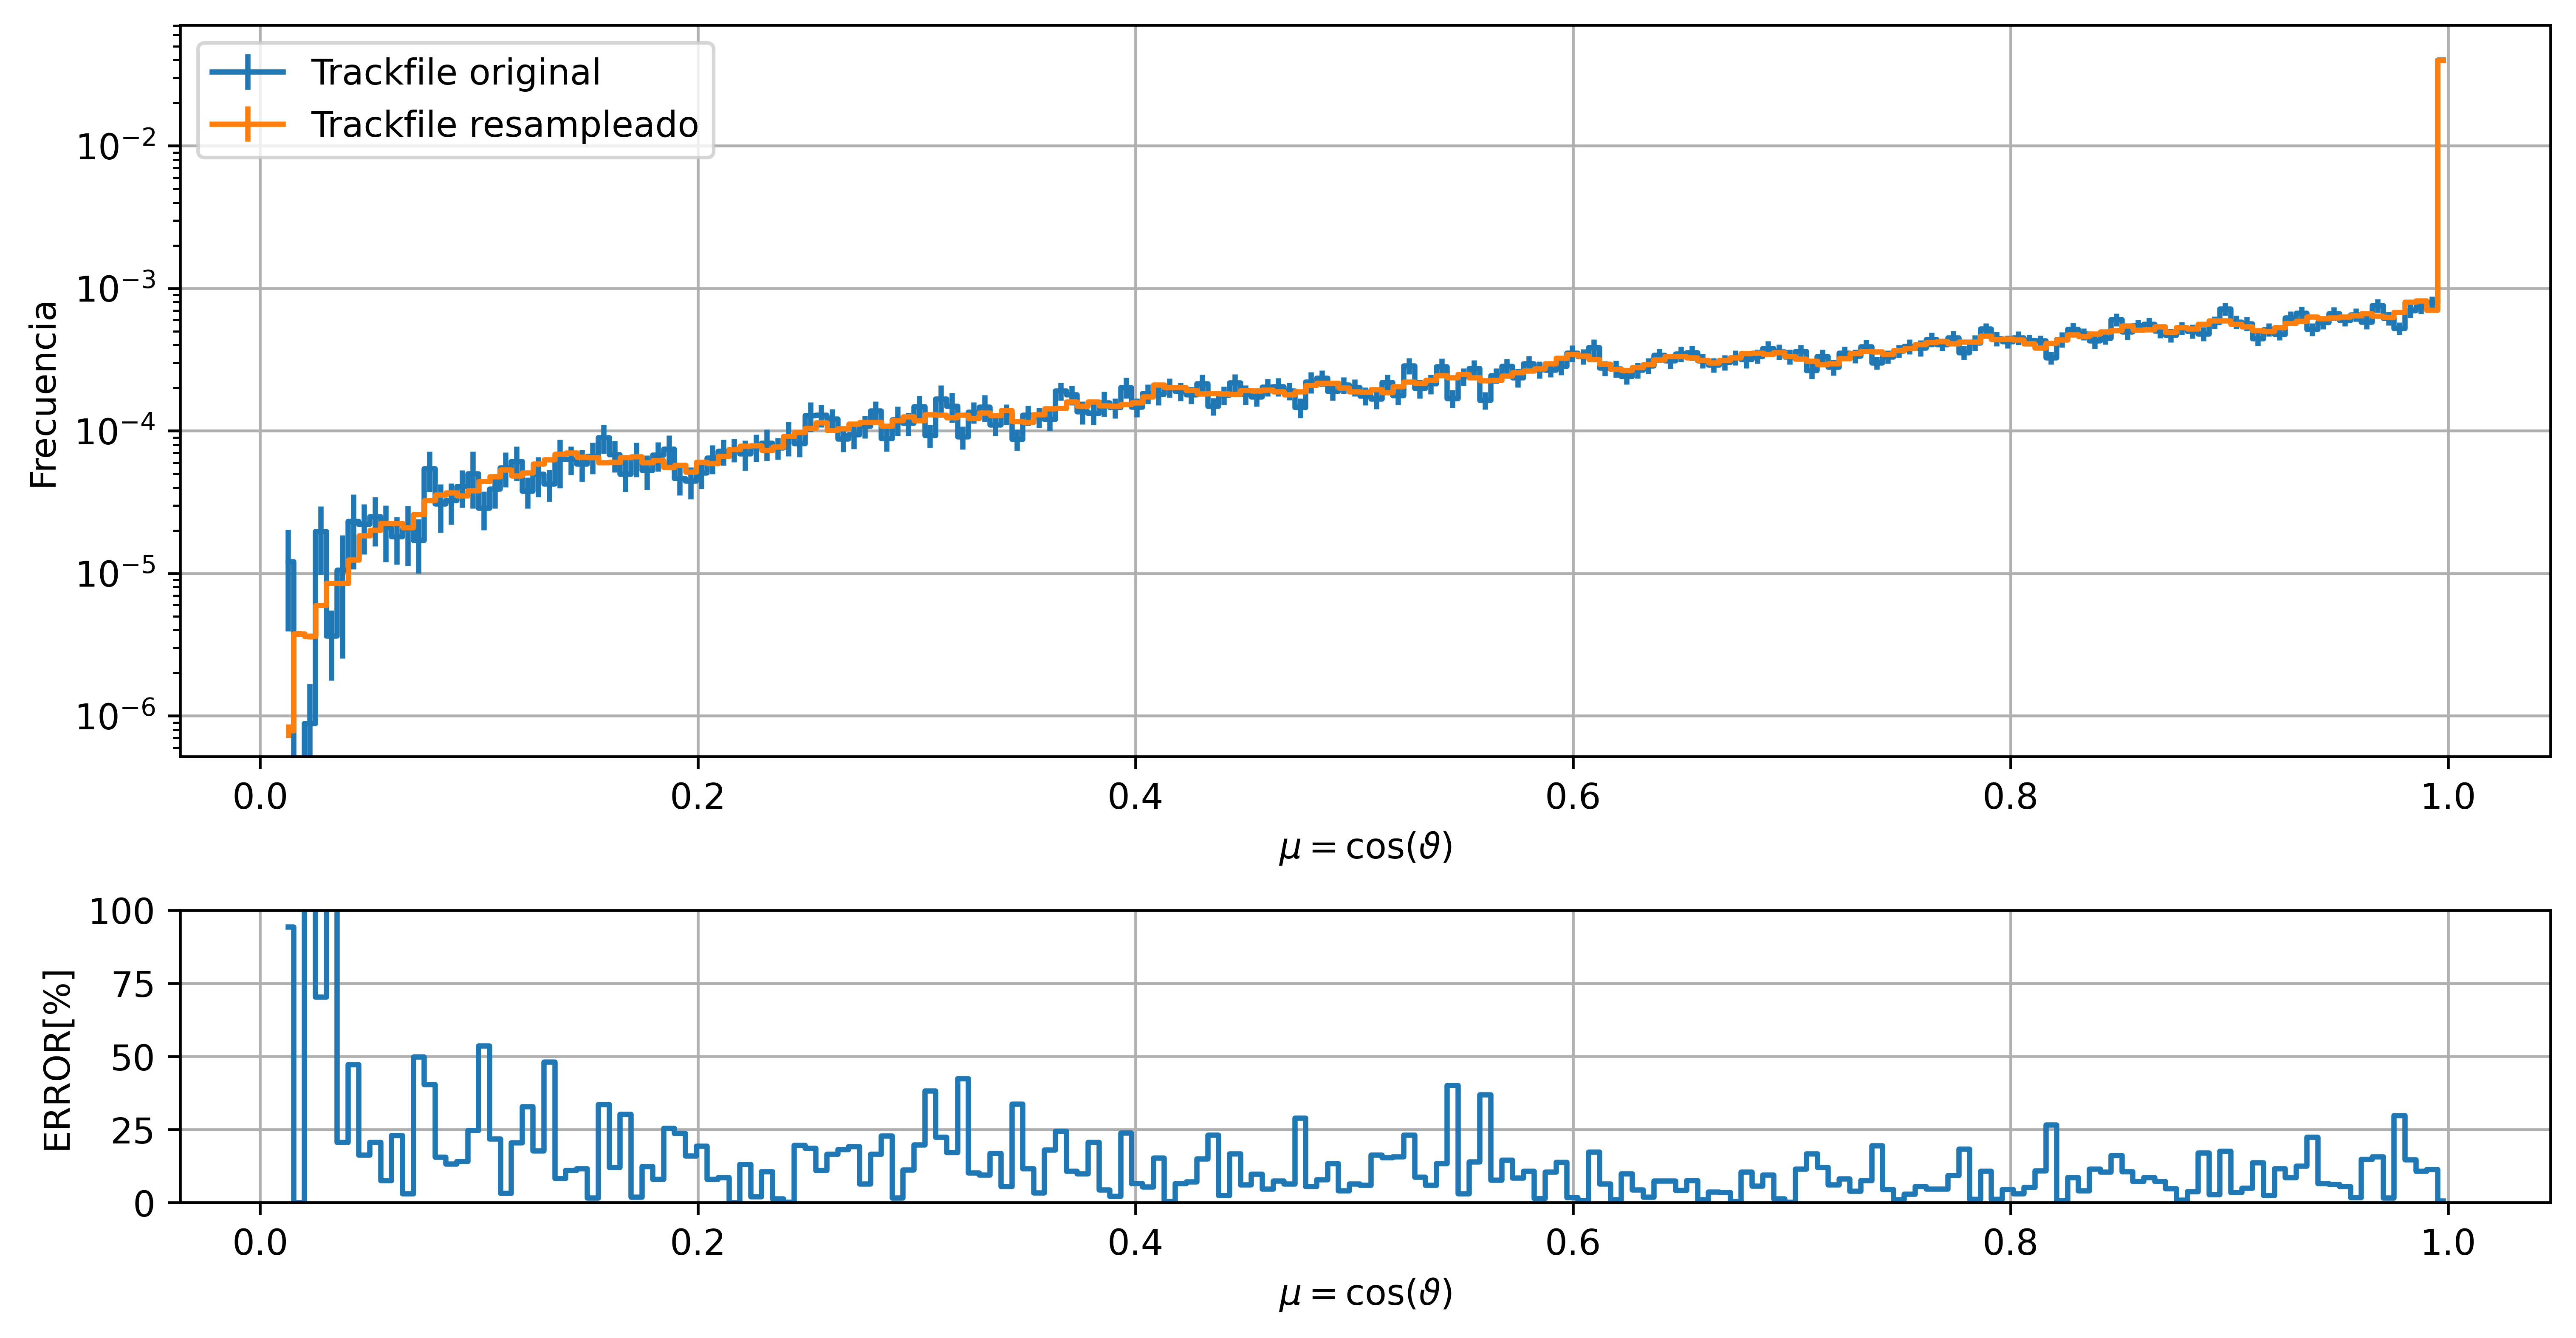
\includegraphics[width=\textwidth]{figs/fig4_8.png}
    \caption{Comparación de la distribución de $\mu$ entre el trackfile original y el trackfile remuestreado. Se observa el efecto de separar manualmente los neutrones con $\mu = 1$.}
    \label{fig:trackfile1_config1_mu_manual}
\end{figure}

A su vez en el grafico 2D de x vs y se observa que la distribucion del canal de vacio se mantiene mas concentrada y no se difumina en el agua. Sin embargo sigue habiendo una forma de cruz en el agua. Esto se sigue debiendo a la discretizacion uniforme de macrogupos. Para solucionar esto deberia haber mas macrogrupos cerca de la interface y menos cerca del borde del modelo, acorde a la cantida de estadistica presente en el \emph{trackfile} original. En la figura \ref{fig:trackfile1_x_y_uniforme_manual} se observa la distribucion de $x$ vs $y$ para el \emph{trackfile} remuestreado utilizando discretizacion uniforme tanto para macrogrupos como para microgrupos, pero con bordes manuales. 

\begin{figure}[H]
    \centering
    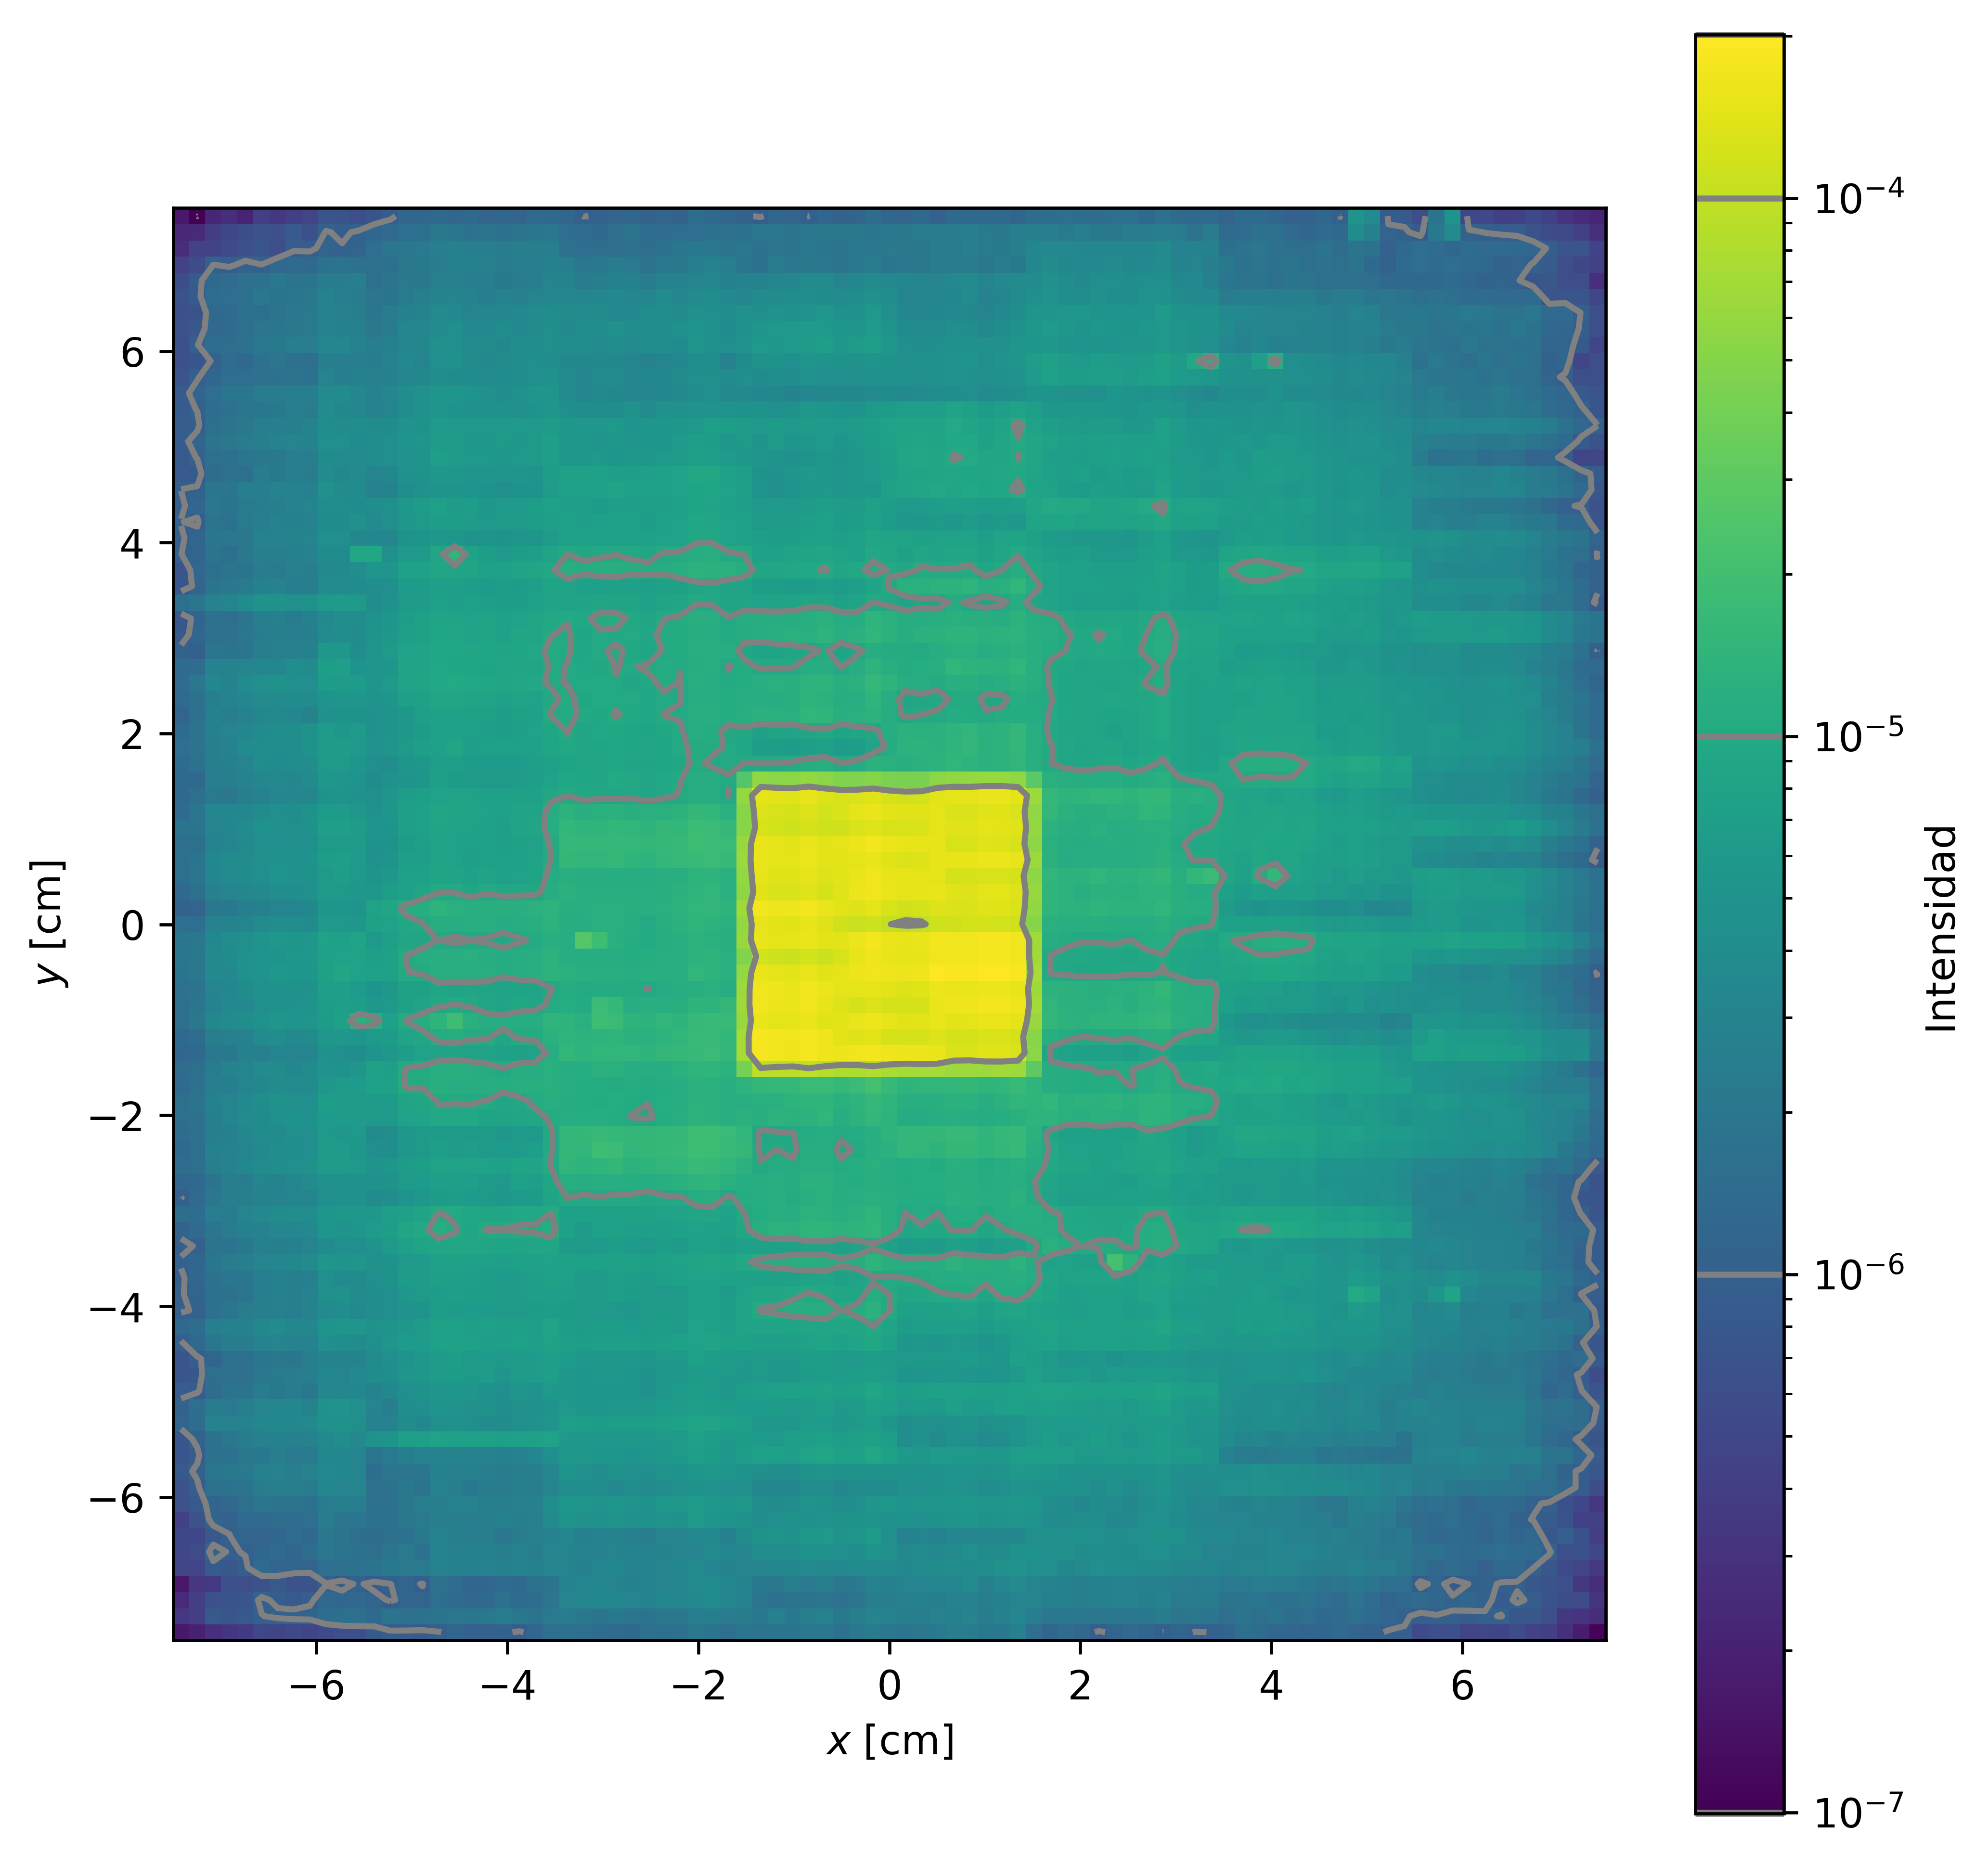
\includegraphics[width=0.75\textwidth]{figs/fig4_9.png}
    \caption{Distribuciones de $x$ vs $y$ para el \emph{trackfile} remuestreado utilizando bordes manuales para separar el canal de vacio explicitamente.}
    \label{fig:trackfile1_x_y_uniforme_manual}
\end{figure}

% \begin{figure}[H]
%     \centering
%     \includegraphics[width=0.7\textwidth]{figuras/macrobordes_configuraciones.pdf}
%     \caption{Esquemas de segmentación para los casos A, B y C.}
%     \label{fig:macrobordes}
% \end{figure}

En la tabla \ref{tab:KL_parciales_equal_columns_manual} se presentan las divergencias KL 1D y 2D, tanto de forma parcial como total, para la configuración de bineado uniforme con bordes manuales. Comparando estos valores contra los valores de la tabla \ref{tab:KL_parciales_equal_columns} referidos a la configuracion de bineado uniforme sin bordes manuales, se observa que la divergencia KL ha disminuido en todos los casos. Esto indica que la segmentación manual de los bordes de los macrogrupos ha permitido mejorar la representación de las distribuciones y correlaciones originales. Los valores mas destacados son los que contienen a la letargia y $\mu$, debido a que concentraban la mayor estadistica.

\begin{table}[H]
    \centering
    \caption{Divergencia KL parcial y total para la configuración \texttt{Equal / Equal}.}
    \label{tab:KL_KL_parciales_equal_columns_manual}
    \begin{tabular}{ll@{\hspace{2cm}}ll}
    \toprule
    \multicolumn{2}{c}{\textbf{KL 1D}} & \multicolumn{2}{c}{\textbf{KL 2D}} \\
    \cmidrule(lr){1-2} \cmidrule(lr){3-4}
    \textbf{Parámetro} & \textbf{Valor} & \textbf{Parámetros} & \textbf{Valor} \\
    \midrule
    $\ln(E_0/E)$ & 5.4229e-01 & $\ln(E_0/E), x$ & 2.7811e+00 \\
    $x$ & 3.3431e-01 & $\ln(E_0/E), y$ & 2.7587e+00 \\
    $y$ & 3.4260e-01 & $\ln(E_0/E), \mu$ & 1.1715e+01 \\
    $\mu$ & 1.3672e+01 & $\ln(E_0/E), \phi$ & 2.4997e+00 \\
    $\phi$ & 4.1083e-01 & $x, y$ & 2.4264e+00 \\
    & & $x, \mu$ & 1.1357e+01 \\
    & & $x, \phi$ & 2.1108e+00 \\
    & & $y, \mu$ & 1.1365e+01 \\
    & & $y, \phi$ & 2.0767e+00 \\
    & & $\mu, \phi$ & 1.1336e+01 \\
    \midrule
    \textbf{Suma KL 1D} & \textbf{1.5302e+01} & \textbf{Suma KL 2D} & \textbf{6.0426e+01} \\
    \bottomrule
    \end{tabular}
    \vspace{0.5em}
    
    KL total = 7.5728e+01
\end{table}

\subsection{Bineado adaptativo de microgrupos y macrogrupos}

Posteriormente se aplicó un esquema de histogramas adaptativos, donde la subdivisión de los macrogrupos fue determinada de forma automática en función de la densidad estadística. Esta técnica permitió una segmentación más eficiente, sin requerir intervención manual del usuario para indicar los cambios bruscos más representativos.

Para obtener una comparacion representativa contra el caso de bineado uniforme, se utilizó la misma cantidad de macrogrupos y microgrupos que en la configuración anterior. En este caso, se emplearon $n_{\text{macro}} = 6$ y $n_{\text{micro}} = 50$ para cada variable, en el orden de variables: \texttt{[ln(E0/E), x, y, mu, phi]}.

Analizando la distribucion remuestreada de letargia y mu podemos ver que se obtiene una densidad de bines mayor en las regiones donde hay mayor estadistica. En la figura \ref{fig:trackfile1_config1_letargia_adaptativo} se observa que la distribucion remuestrada conserva la delta en letargia minima y se le asignan mas bines a la zona de letargia baja y termalizacion. A su vez se observa que se asignan relativamente pocos bines en donde hay pocos bines, provocando una mayor suavidad. En la figura \ref{fig:trackfile1_config1_mu_adaptativo} se observa que la distribucion remuestrada conserva la delta en $\mu = 1$ y se le asignan mas bines a la zona de $\mu = 1$. Sin embargo se observa que se reproduce el ruido estadistico debido a que hay un exceso de micro bines. 

\begin{figure}[H]
    \centering
    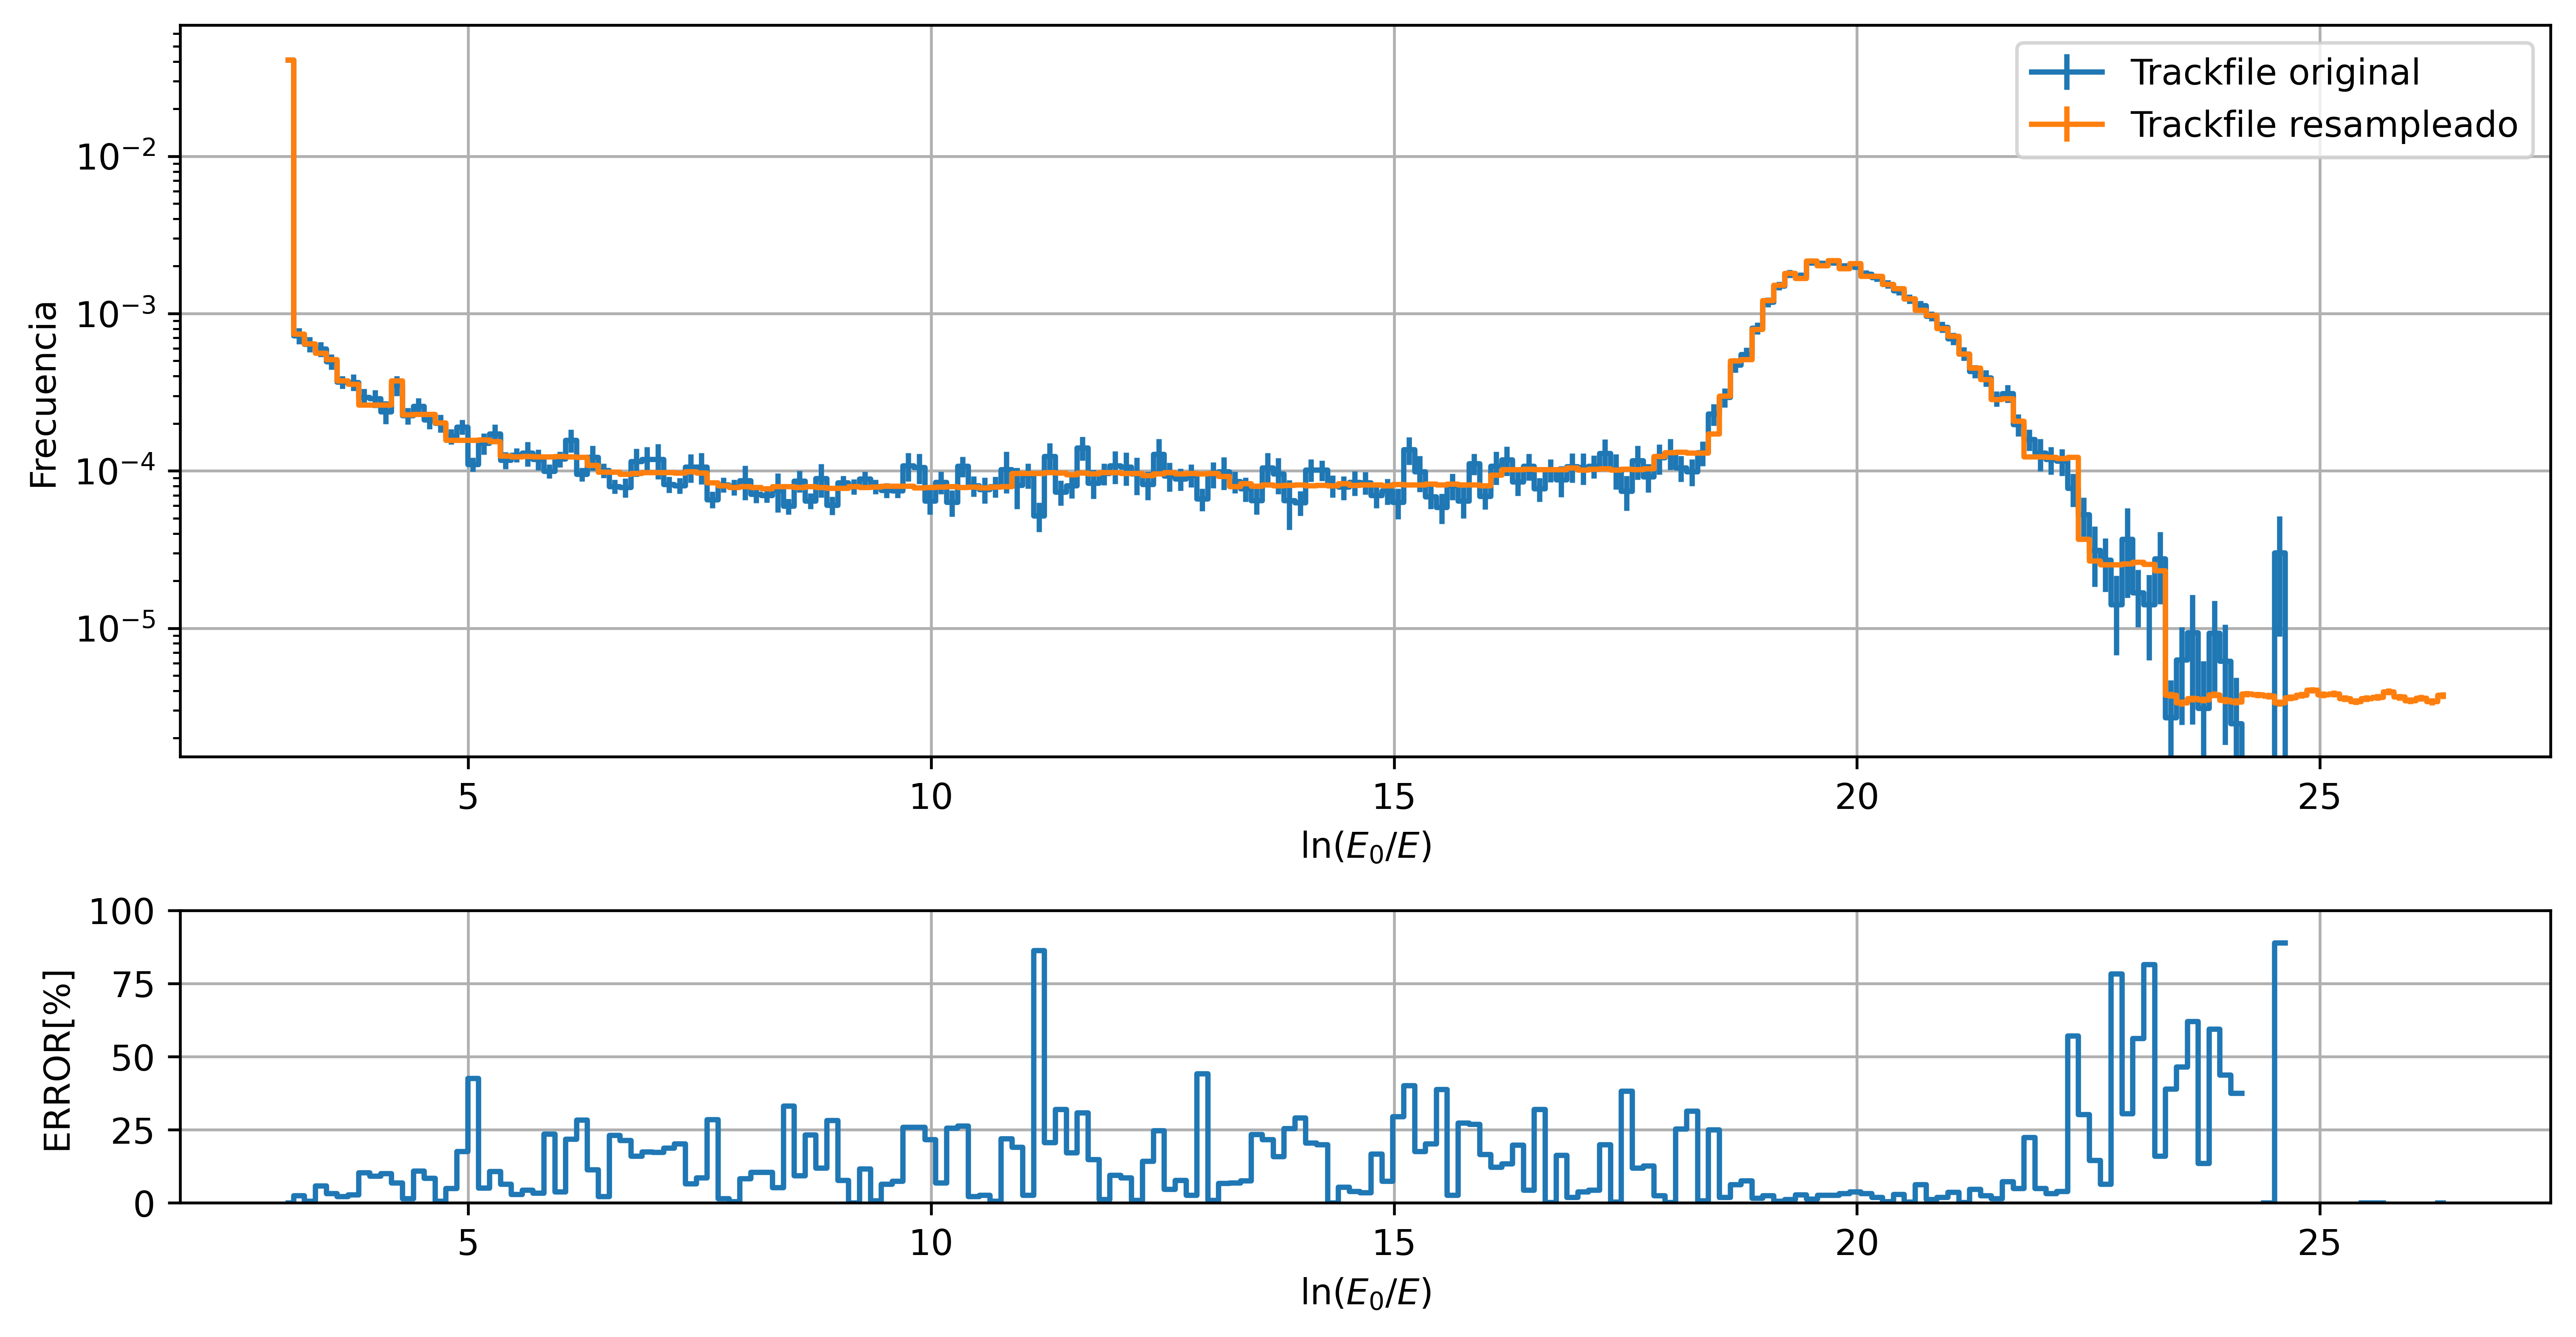
\includegraphics[width=\textwidth]{figs/fig4_10.png}
    \caption{Comparación de la distribución de letargia entre el trackfile original y el trackfile remuestreado.}
    \label{fig:trackfile1_config1_letargia_adaptativo}
\end{figure}

\begin{figure}[H]
    \centering
    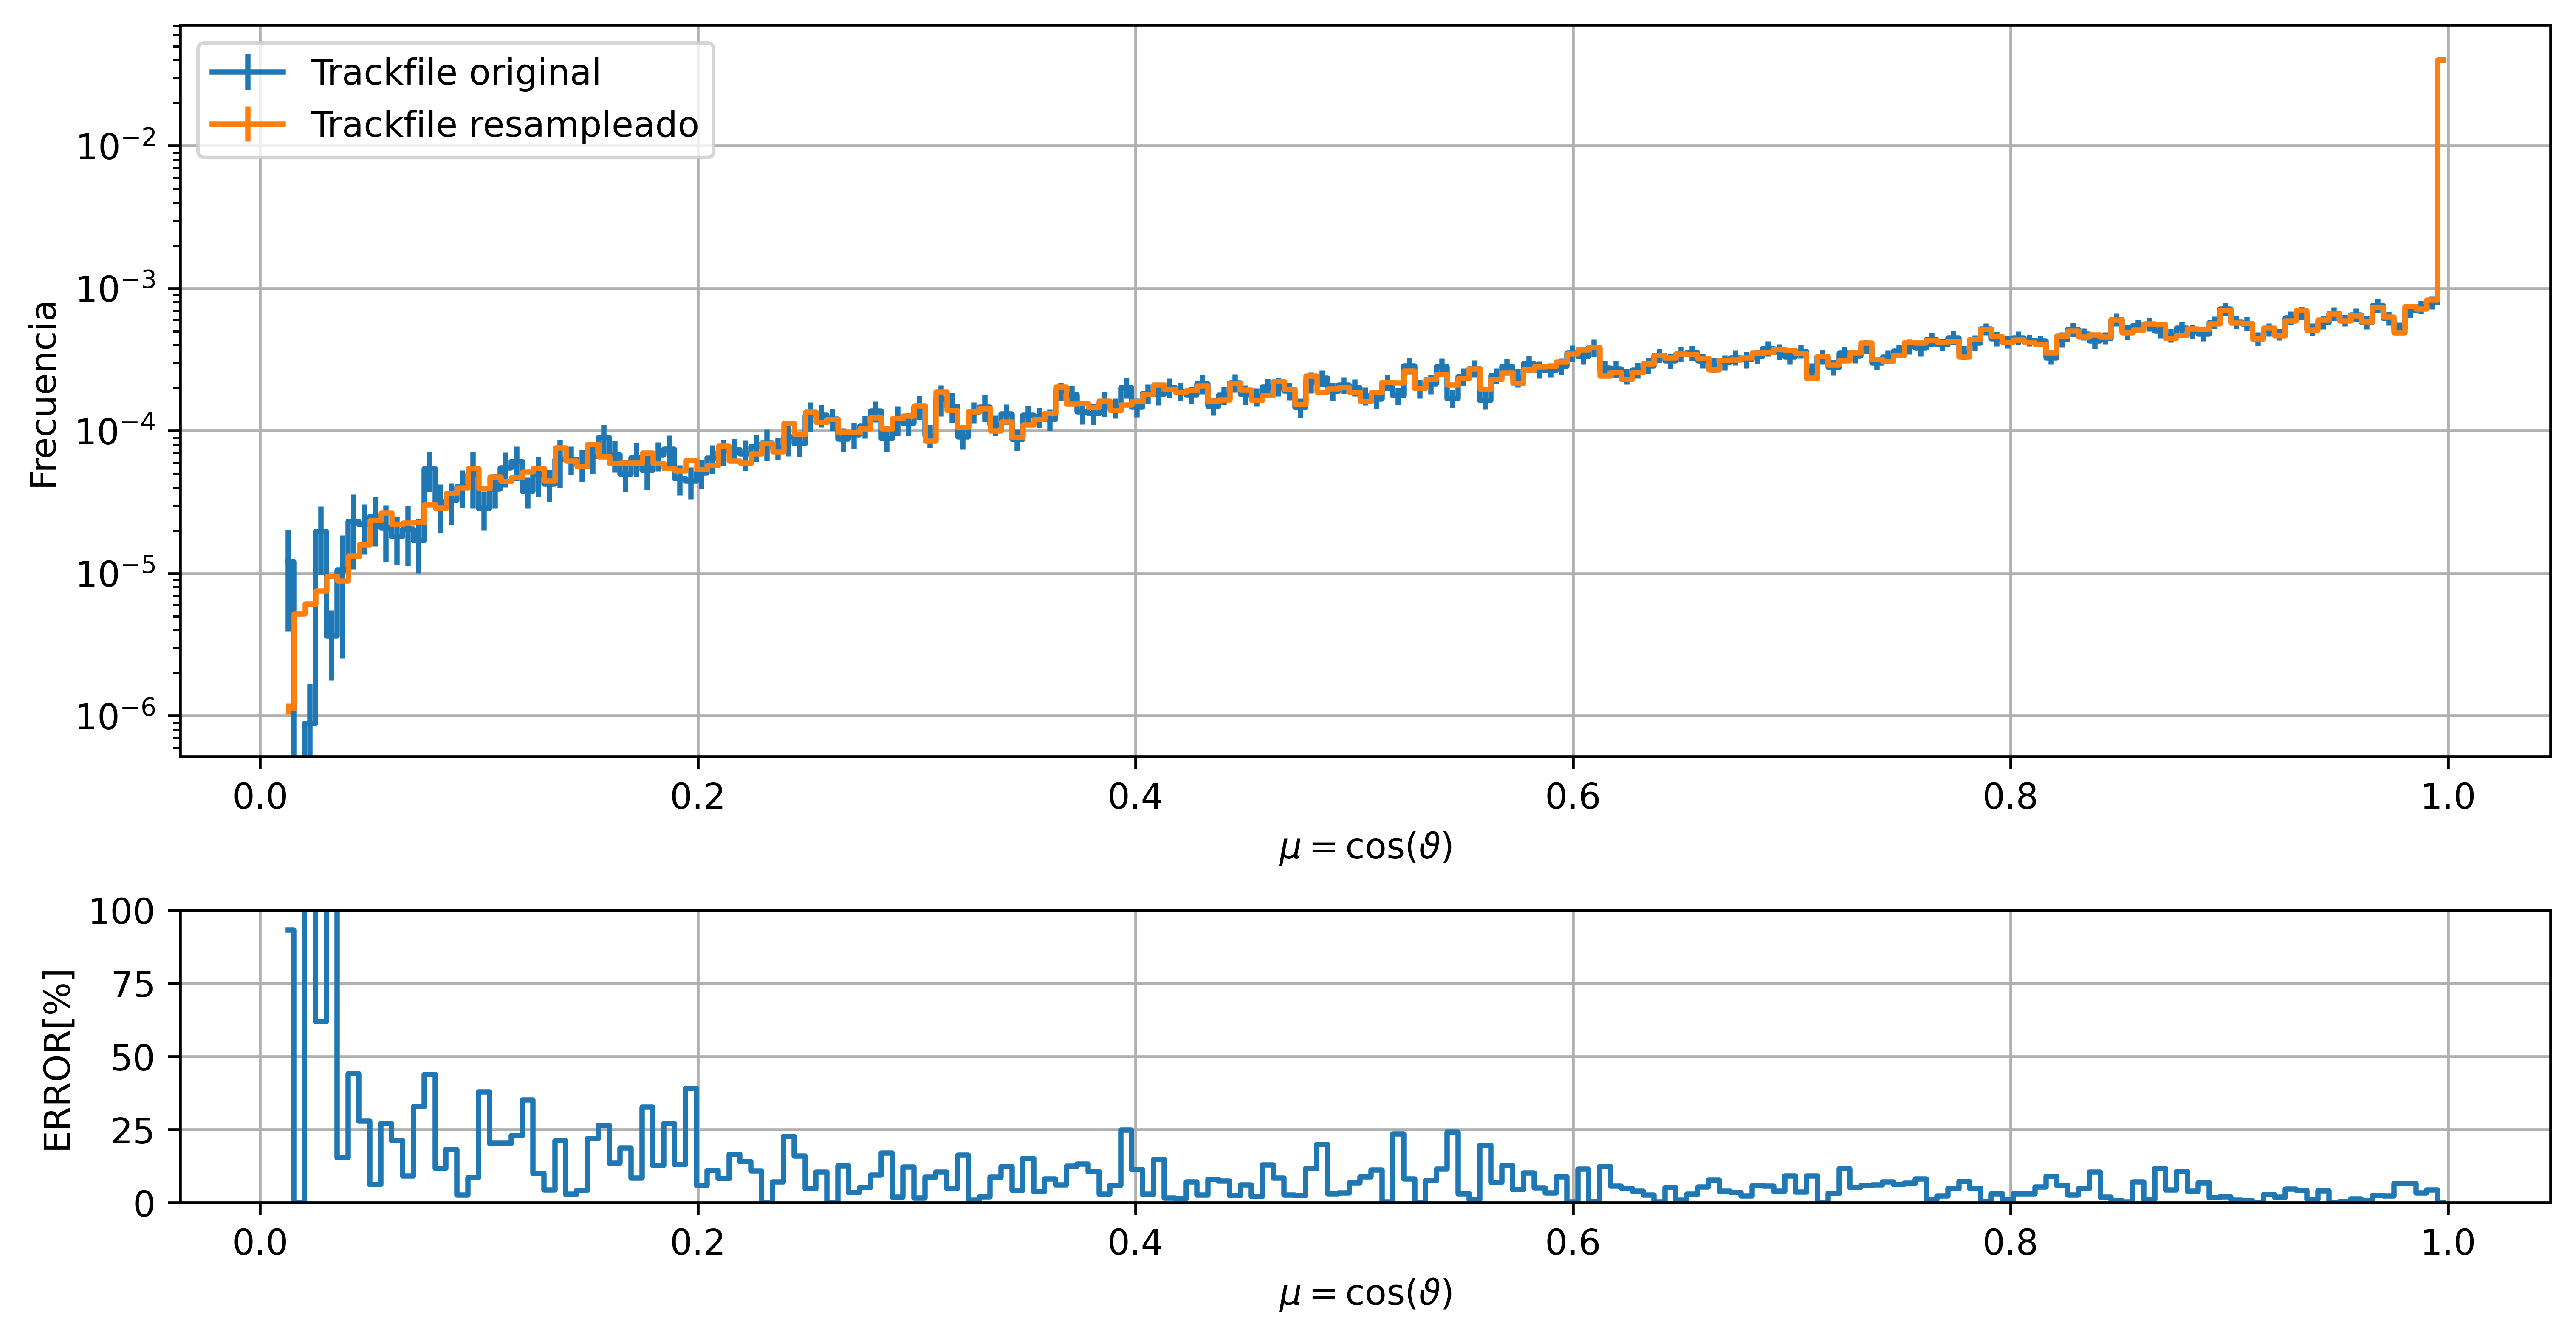
\includegraphics[width=\textwidth]{figs/fig4_11.png}
    \caption{Comparación de la distribución de $\mu$ entre el trackfile original y el trackfile remuestreado.}
    \label{fig:trackfile1_config1_mu_adaptativo}
\end{figure}

Observando la distribucion remuestreada de x vs y  graficada en la figura \ref{fig:trackfile1_x_y_uniforme_adaptativo} se observa que la distribucion del canal de vacio se mantiene mas concentrada y no se difumina en el agua. A su vez se observa que la distribucion del agua se mantiene mas difusa y no se observa la forma de cruz que se observaba en el caso de bineado uniforme. Esto es debido a que al ser un bineado adaptativo, los bines se asignan donde hay mayor estadistica, evitando formar grupos de neutrones con poca estadistica.

\begin{figure}[H]
    \centering
    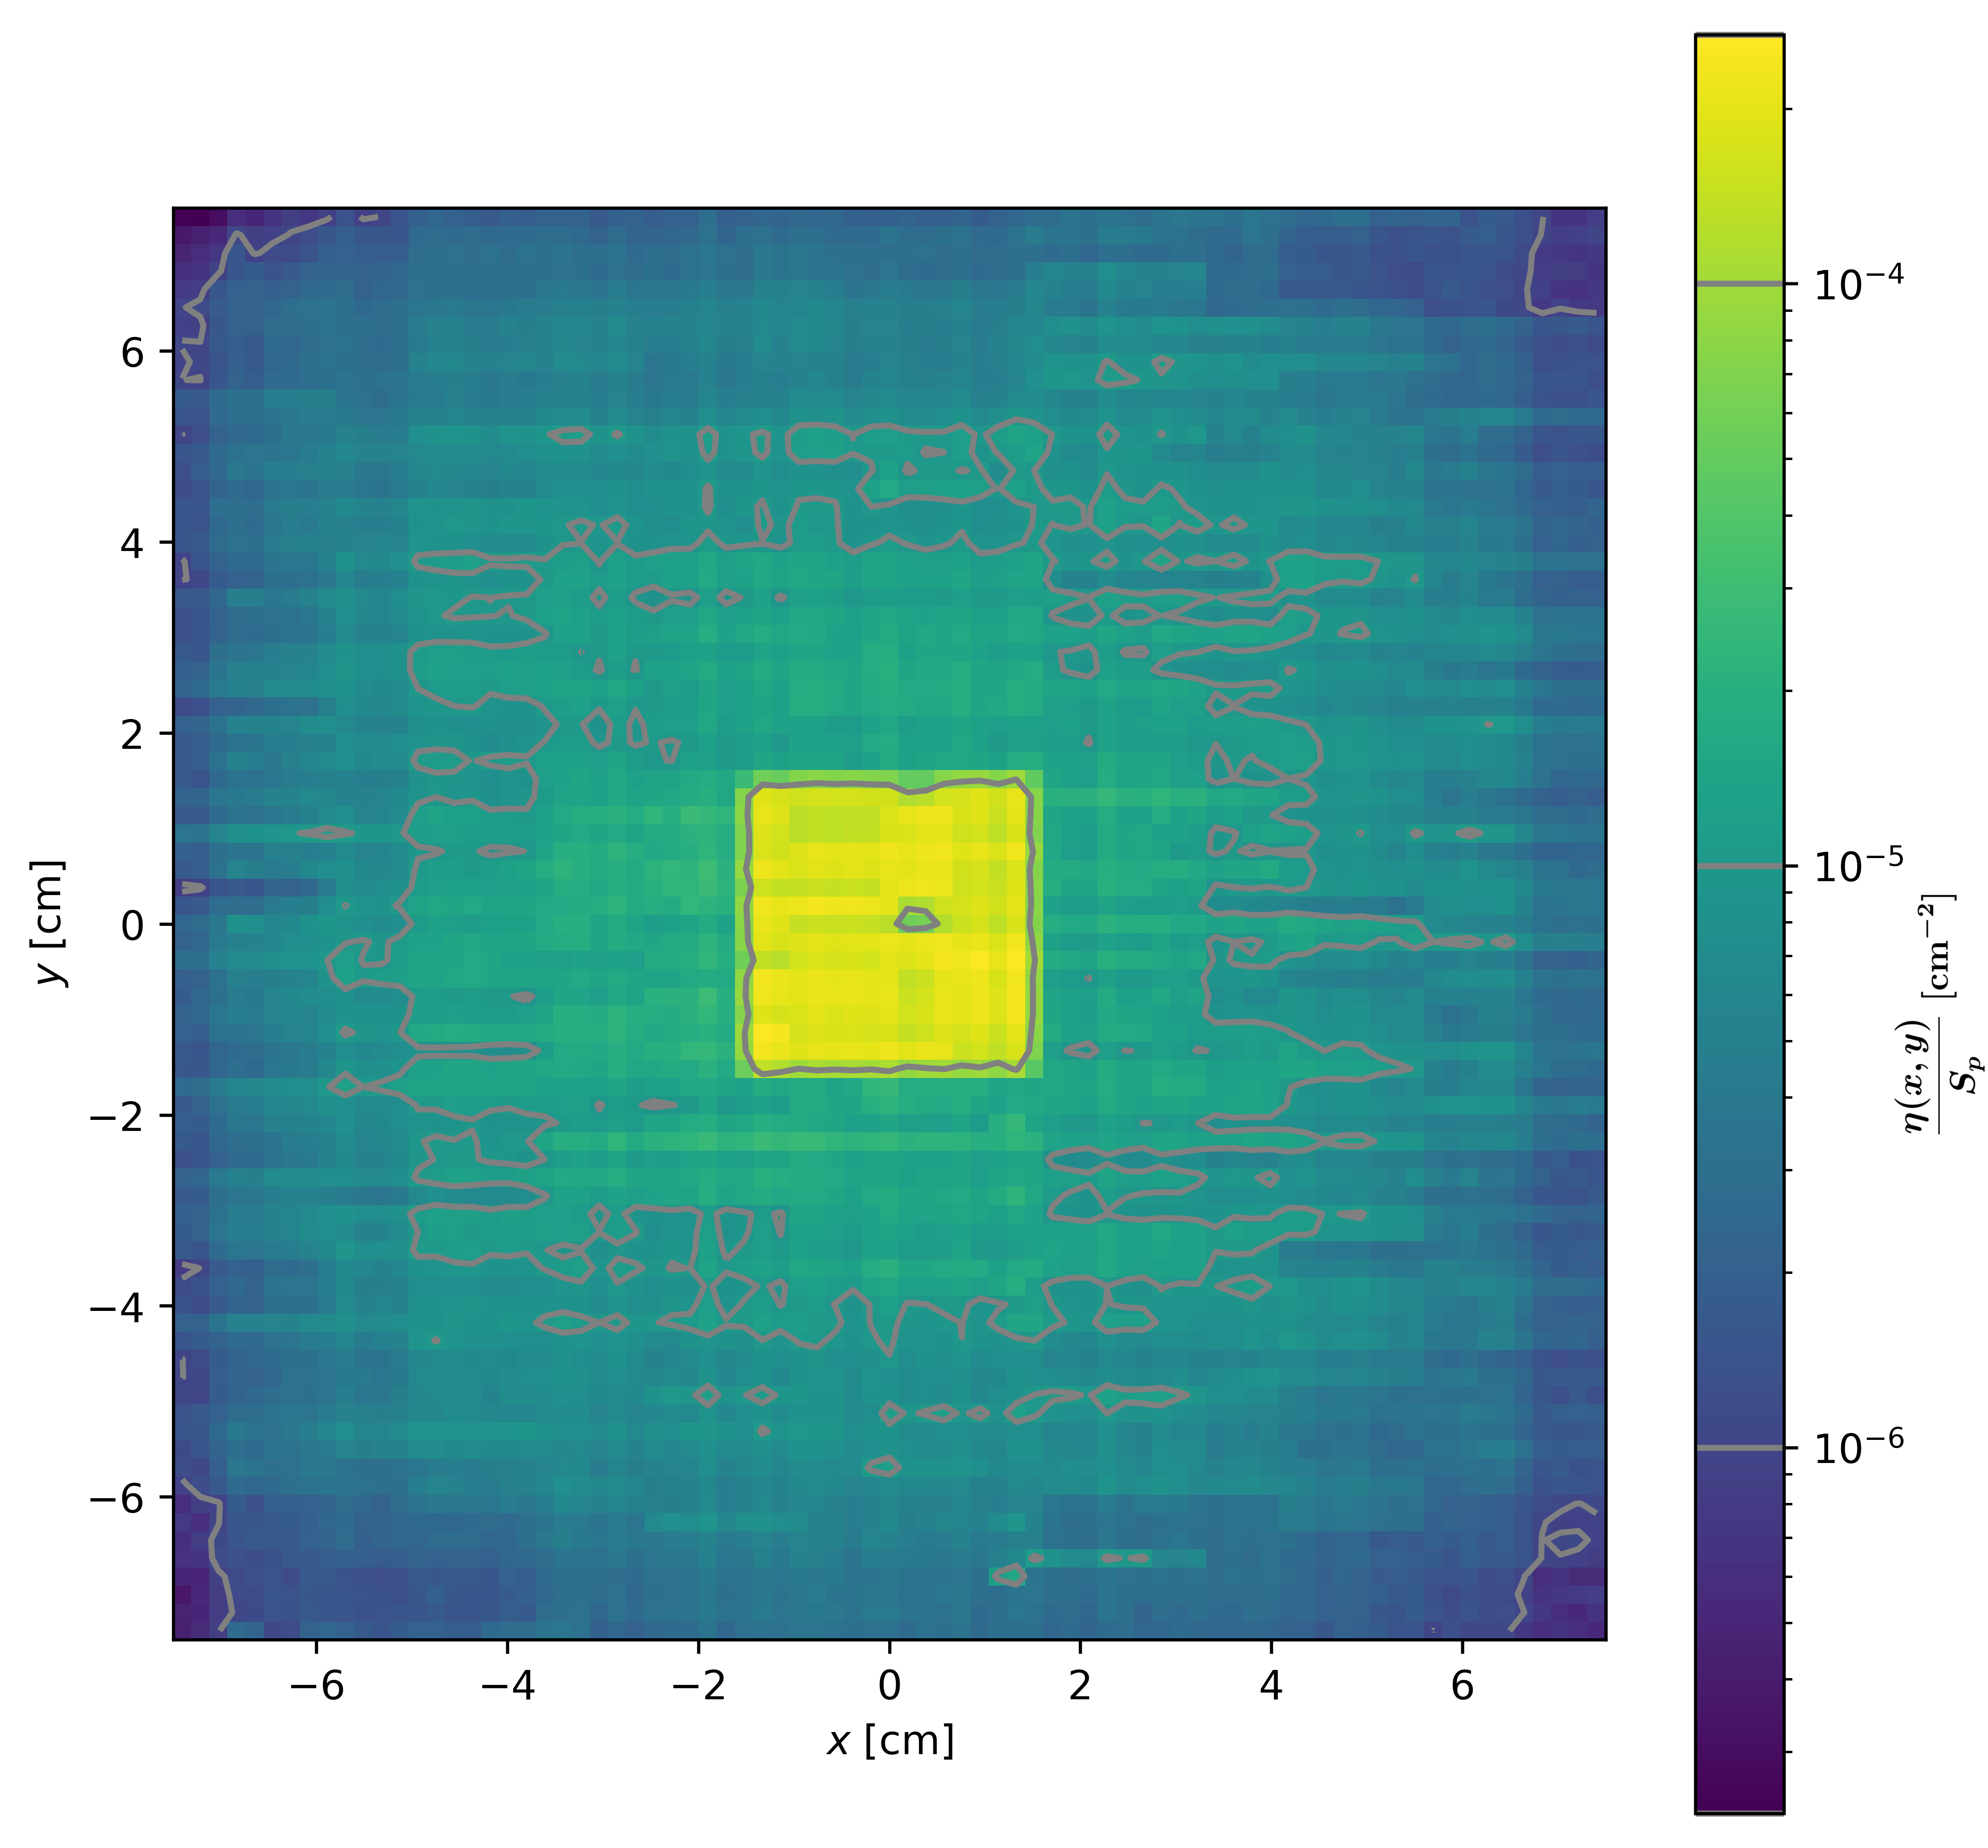
\includegraphics[width=0.75\textwidth]{figs/fig4_12.png}
    \caption{Distribuciones de $x$ vs $y$ para el \emph{trackfile} remuestreado.}
    \label{fig:trackfile1_x_y_uniforme_adaptativo}
\end{figure}

En la tabla \ref{tab:KL_parciales_adaptativo} se presentan las divergencias KL 1D y 2D, tanto de forma parcial como total, para la configuración de bineado adaptativo. Comparando estos valores contra los valores de la tabla \ref{tab:KL_parciales_equal_columns_manual} referidos a la configuracion de bineado uniforme con bordes manuales, se observa que se obtiene una metrica KL similar al caso de bineado uniforme con bordes manuales. 

\begin{table}[H]
    \centering
    \caption{Divergencia KL parcial y total para la configuración \texttt{Equal / Equal}.}
    \label{tab:KL_parciales_adaptativo}
    \begin{tabular}{ll@{\hspace{2cm}}ll}
    \toprule
    \multicolumn{2}{c}{\textbf{KL 1D}} & \multicolumn{2}{c}{\textbf{KL 2D}} \\
    \cmidrule(lr){1-2} \cmidrule(lr){3-4}
    \textbf{Parámetro} & \textbf{Valor} & \textbf{Parámetros} & \textbf{Valor} \\
    \midrule
    $\ln(E_0/E)$ & 5.4758e-01 & $\ln(E_0/E), x$ & 2.8433e+00 \\
    $x$ & 3.4476e-01 & $\ln(E_0/E), y$ & 2.9157e+00 \\
    $y$ & 3.5721e-01 & $\ln(E_0/E), \mu$ & 1.1745e+01 \\
    $\mu$ & 1.3679e+01 & $\ln(E_0/E), \phi$ & 3.8279e+00 \\
    $\phi$ & 4.3238e-01 & $x, y$ & 2.7147e+00 \\
    & & $x, \mu$ & 1.1421e+01 \\
    & & $x, \phi$ & 3.1527e+00 \\
    & & $y, \mu$ & 1.1436e+01 \\
    & & $y, \phi$ & 3.0822e+00 \\
    & & $\mu, \phi$ & 1.1630e+01 \\
    \midrule
    \textbf{Suma KL 1D} & \textbf{1.5361e+01} & \textbf{Suma KL 2D} & \textbf{6.4769e+01} \\
    \bottomrule
    \end{tabular}
    \vspace{0.5em}
    
    KL total = 8.0129e+01
\end{table}



% Los resultados mostraron una mejora significativa en la reconstrucción de las distribuciones 1D y 2D, así como en las métricas de error globales como la divergencia de Kullback-Leibler (KL) y el error medio absoluto.

% \begin{figure}[H]
%     \centering
%     \includegraphics[width=0.48\textwidth]{figuras/rel_error_adaptativo_2D.pdf}
%     \includegraphics[width=0.48\textwidth]{figuras/KL_vs_metodo.pdf}
%     \caption{Izq: error relativo en plano $\mu$ vs.\ letargia. Der: comparación de KL entre métodos.}
%     \label{fig:adaptativo-resultados}
% \end{figure}

\subsection{Bineado adaptativo de microgrupos y macrogrupos optimizado}
Debido a que la seccion anterior mostro que se obtiene una mejor utilizacion de los bines al utilizar un bineado adaptativo, se decidio seguir trabajando con este metodo y optimizar la cantidad de microgrupos y macrogrupos. Es posible aumentar la cantidad de macrogrupos y disminuir la cantidad de microgrupos, obteniendo una mejor representacion de las correlaciones y una distribucion de las variables mas suavizada en las regiones de menor estadistica. A su vez es posible utilizar una cantidad de macrogrupos y microgrupos distinta para cada variable. 

Se utilizo la siguiente configuracion de macrogrupos y microgrupos:
\begin{itemize}
    \item \textbf{Macrogrupos:} se utilizo la configuracion [6, 6, 6, 6, 6].
    \item \textbf{Microgrupos:} se utilizo la configuracion [50, 50, 50, 50, 50].
\end{itemize}

\section{Resultados de la simulación comparativa}
\subsection{Validación de tallies y aplicación de técnicas de reducción de varianza}

Para validar los resultados se evaluaron distintas magnitudes físicas a lo largo del eje del sistema:

\begin{itemize}
    \item Flujo escalar en secciones transversales: total, en agua, y en vacío.
    \item Espectro energético sobre una superficie de tally a $z = 80\,\text{cm}$.
    \item Corriente en dirección $z$ sobre planos intermedios.
\end{itemize}

Se aplicó reducción de varianza mediante weight windows generados con OpenMC, especialmente en regiones con moderación intensa, lo cual mejoró la estadística de tallies en el agua sin alterar el resultado global.

% \begin{figure}[H]
%     \centering
%     \includegraphics[width=0.65\textwidth]{figuras/flujo_vs_z_comparacion.pdf}
%     \caption{Flujo escalar promedio a lo largo del canal. Comparación entre simulación original y reconstruida.}
%     \label{fig:flujo-vs-z}
% \end{figure}

\subsection{Síntesis y conclusiones}

El caso del canal de vacío embebido en agua permitió poner en evidencia los desafíos que presentan las técnicas de muestreo cuando coexisten poblaciones de partículas con comportamientos disímiles. Se comprobó que:

\begin{itemize}
    \item La segmentación espacial y direccional es crucial para preservar correlaciones en el muestreo.
    \item Los histogramas adaptativos constituyen una alternativa robusta y automática frente a configuraciones manuales.
    \item El método propuesto reproduce con alta fidelidad los resultados de flujo, espectro y corriente.
\end{itemize}

Este caso sirve como referencia para futuras aplicaciones en geometrías más complejas donde también existan discontinuidades materiales o comportamientos multi-modales del campo de neutrones.

